	%!TEX root = ../template.tex
%%%%%%%%%%%%%%%%%%%%%%%%%%%%%%%%%%%%%%%%%%%%%%%%%%%%%%%%%%%%%%%%%%%%
%% chapter4.tex
%% NOVA thesis document file
%%
%% Chapter with lots of dummy text
%%%%%%%%%%%%%%%%%%%%%%%%%%%%%%%%%%%%%%%%%%%%%%%%%%%%%%%%%%%%%%%%%%%%

\typeout{NT FILE chapter4.tex}%

\chapter{Unveiling the \textit{Grammar} of Time Series}
\label{cha:segmentation}


\begin{figure}
\centering

\includegraphics[width=\linewidth]{ssm_topics.pdf}
\caption{Information retrieval topics explained in this Chapter. Each of these topics is a result of analyzing the \gls{SSM}.}
\label{fig:info_retrieval_topics}
\end{figure}

Researchers are interested in understanding the structure of the recorded signals, the meaning behind them, and the influences of the context. In Chapter 1 (see Section \ref{sub:context1}) we gave several examples of how signals in our everyday life can be structured and partitioned, such as a signal representing a \textcolor{myblue}{walking} regime shifting to a \textcolor{mygreen}{jogging} regime (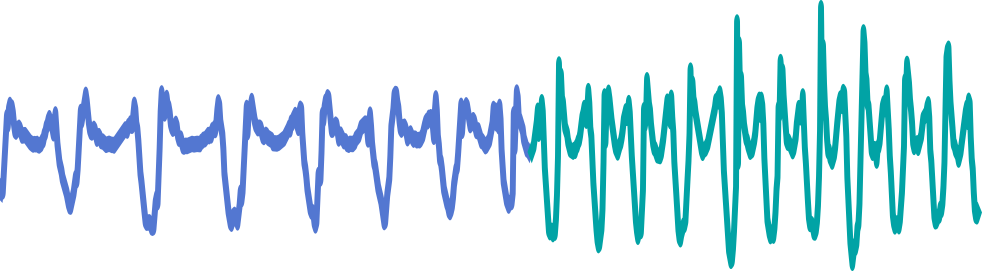
\includegraphics[height=5ex, valign=m]{walking_jogging.png}). The examples we mentioned in Chapter 1 and above manifest the relevance and importance of the following approaches:

\begin{itemize}
     \item \textbf{Novelty segmentation}: to identify significant changes in the signal's behaviour.
    \item \textbf{Periodic segmentation}: to detect the presence of repeating cyclic patterns.
    \item \textbf{Labelling}: to measure how similar the segments are between each other with the help of similarity profiles.
    \item \textbf{Query search}: to find repeating patterns in the time series based on a \textit{subsequence} given as an example.
    \item \textbf{Summarization}: to summarize visually the time series by partitioning it into relevant and uniform/periodic segments and joining segments based on their similarity.
\end{itemize}

In this Chapter, we present the proposed solutions to these five problems mentioned above, inspired by a method used for audio signal analysis and thumbnail generation \cite{fmp1, audiolabs1, audiolabs2, cpd_audio}. Such a method has not yet been extended to other types of \textit{time series} domains that could greatly benefit from it \cite{muller_music_health}. The method uses a feature-based \gls{ssm} of (multidimensional) time series, from which visual and analytical information is rendered to perform the segmentation process and associate \textit{subsequences} of the time series with each other, which forwards automatic labelling and ultimately can be used to summarize the signal. We extended its application to \textit{biosignals} with the usage of general features, and introduced new methods to analyze the \gls{ssm} for periodic segmentation, labelling, query search and summarization.


\section{The Problem}

Defining what is relevant in a time series highly depends on the context and purpose of the analysis, but globally, for any type of time series, there is a general interest in understanding how the signal is structured, especially for tasks related to data annotation/labeling. The structure of a time series is built of \textit{segments} delimited by \textit{events}. The problem explored in this section is the search for such \textit{events} and how to find the ones that are significant. 
\par
From definition 4 of Chapter \ref{sec:global}, we highlight two primary considerations for the detection of events: (1) an event is a change in the behavior of the time series, and (2) it has to be significant both \textit{statistically} and \textit{qualitatively}. The \textit{qualitative} aspect indicates subjectivity from the analyst because of the domain or context of the problem. Considering this, we will start by explaining the dimensions of the problem: (1) search and (2) type of significance. 

\subsection{Search Ranks}

\begin{figure}[H]
    \centering
    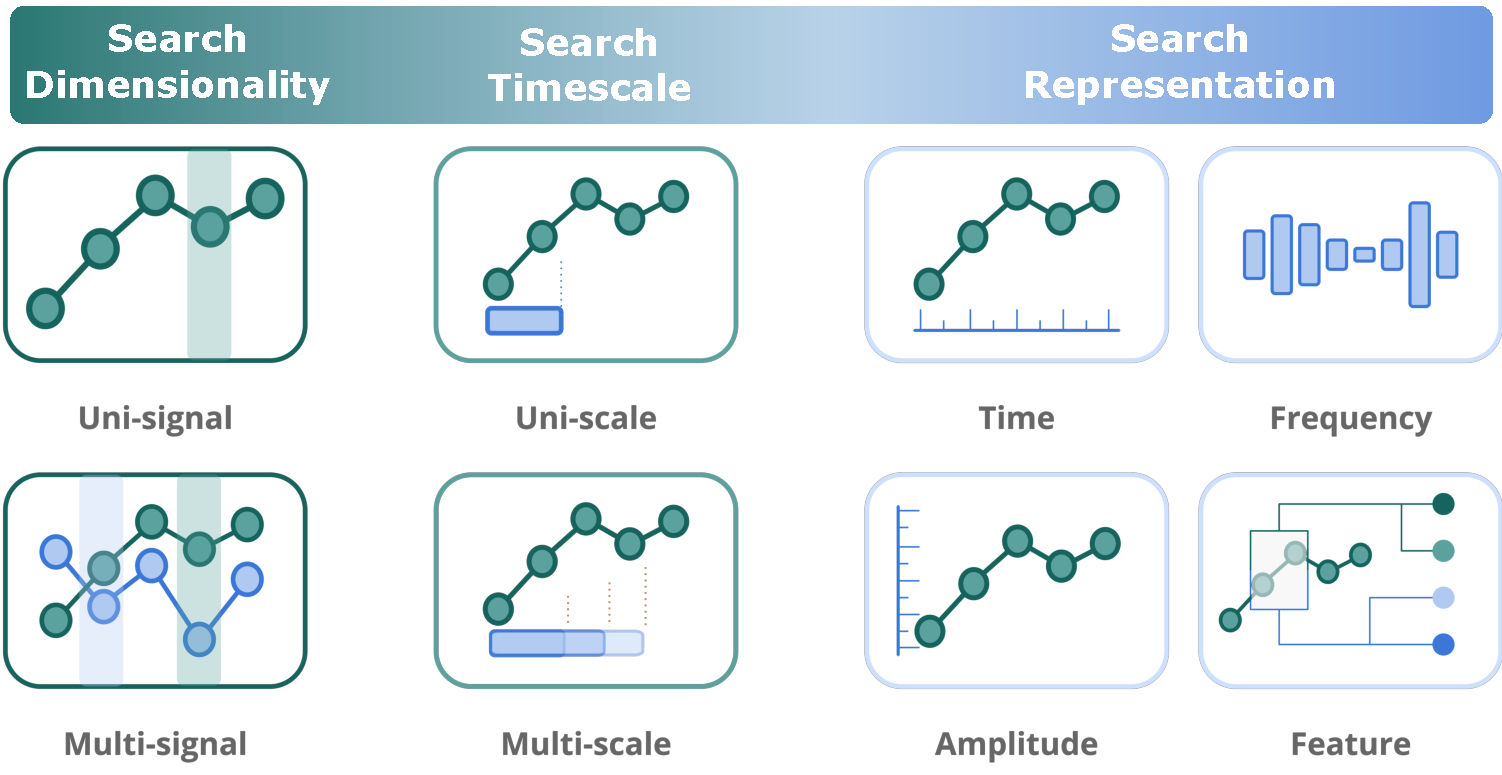
\includegraphics[width=\linewidth]{event_search.pdf}
    \caption{Event search in different ranks of dimensionality, timescales, and representation.}
    \label{fig:event_search}
\end{figure}


%\begin{figure}
%\begin{subfigure}{.5\textwidth}
%	\centering
%	\includegraphics[width=0.95\linewidth]{event_search.png}
%	\label{fig:event_search}
%	\caption{}
%\end{subfigure}%
%\begin{subfigure}{.5\textwidth}
%	\centering
%	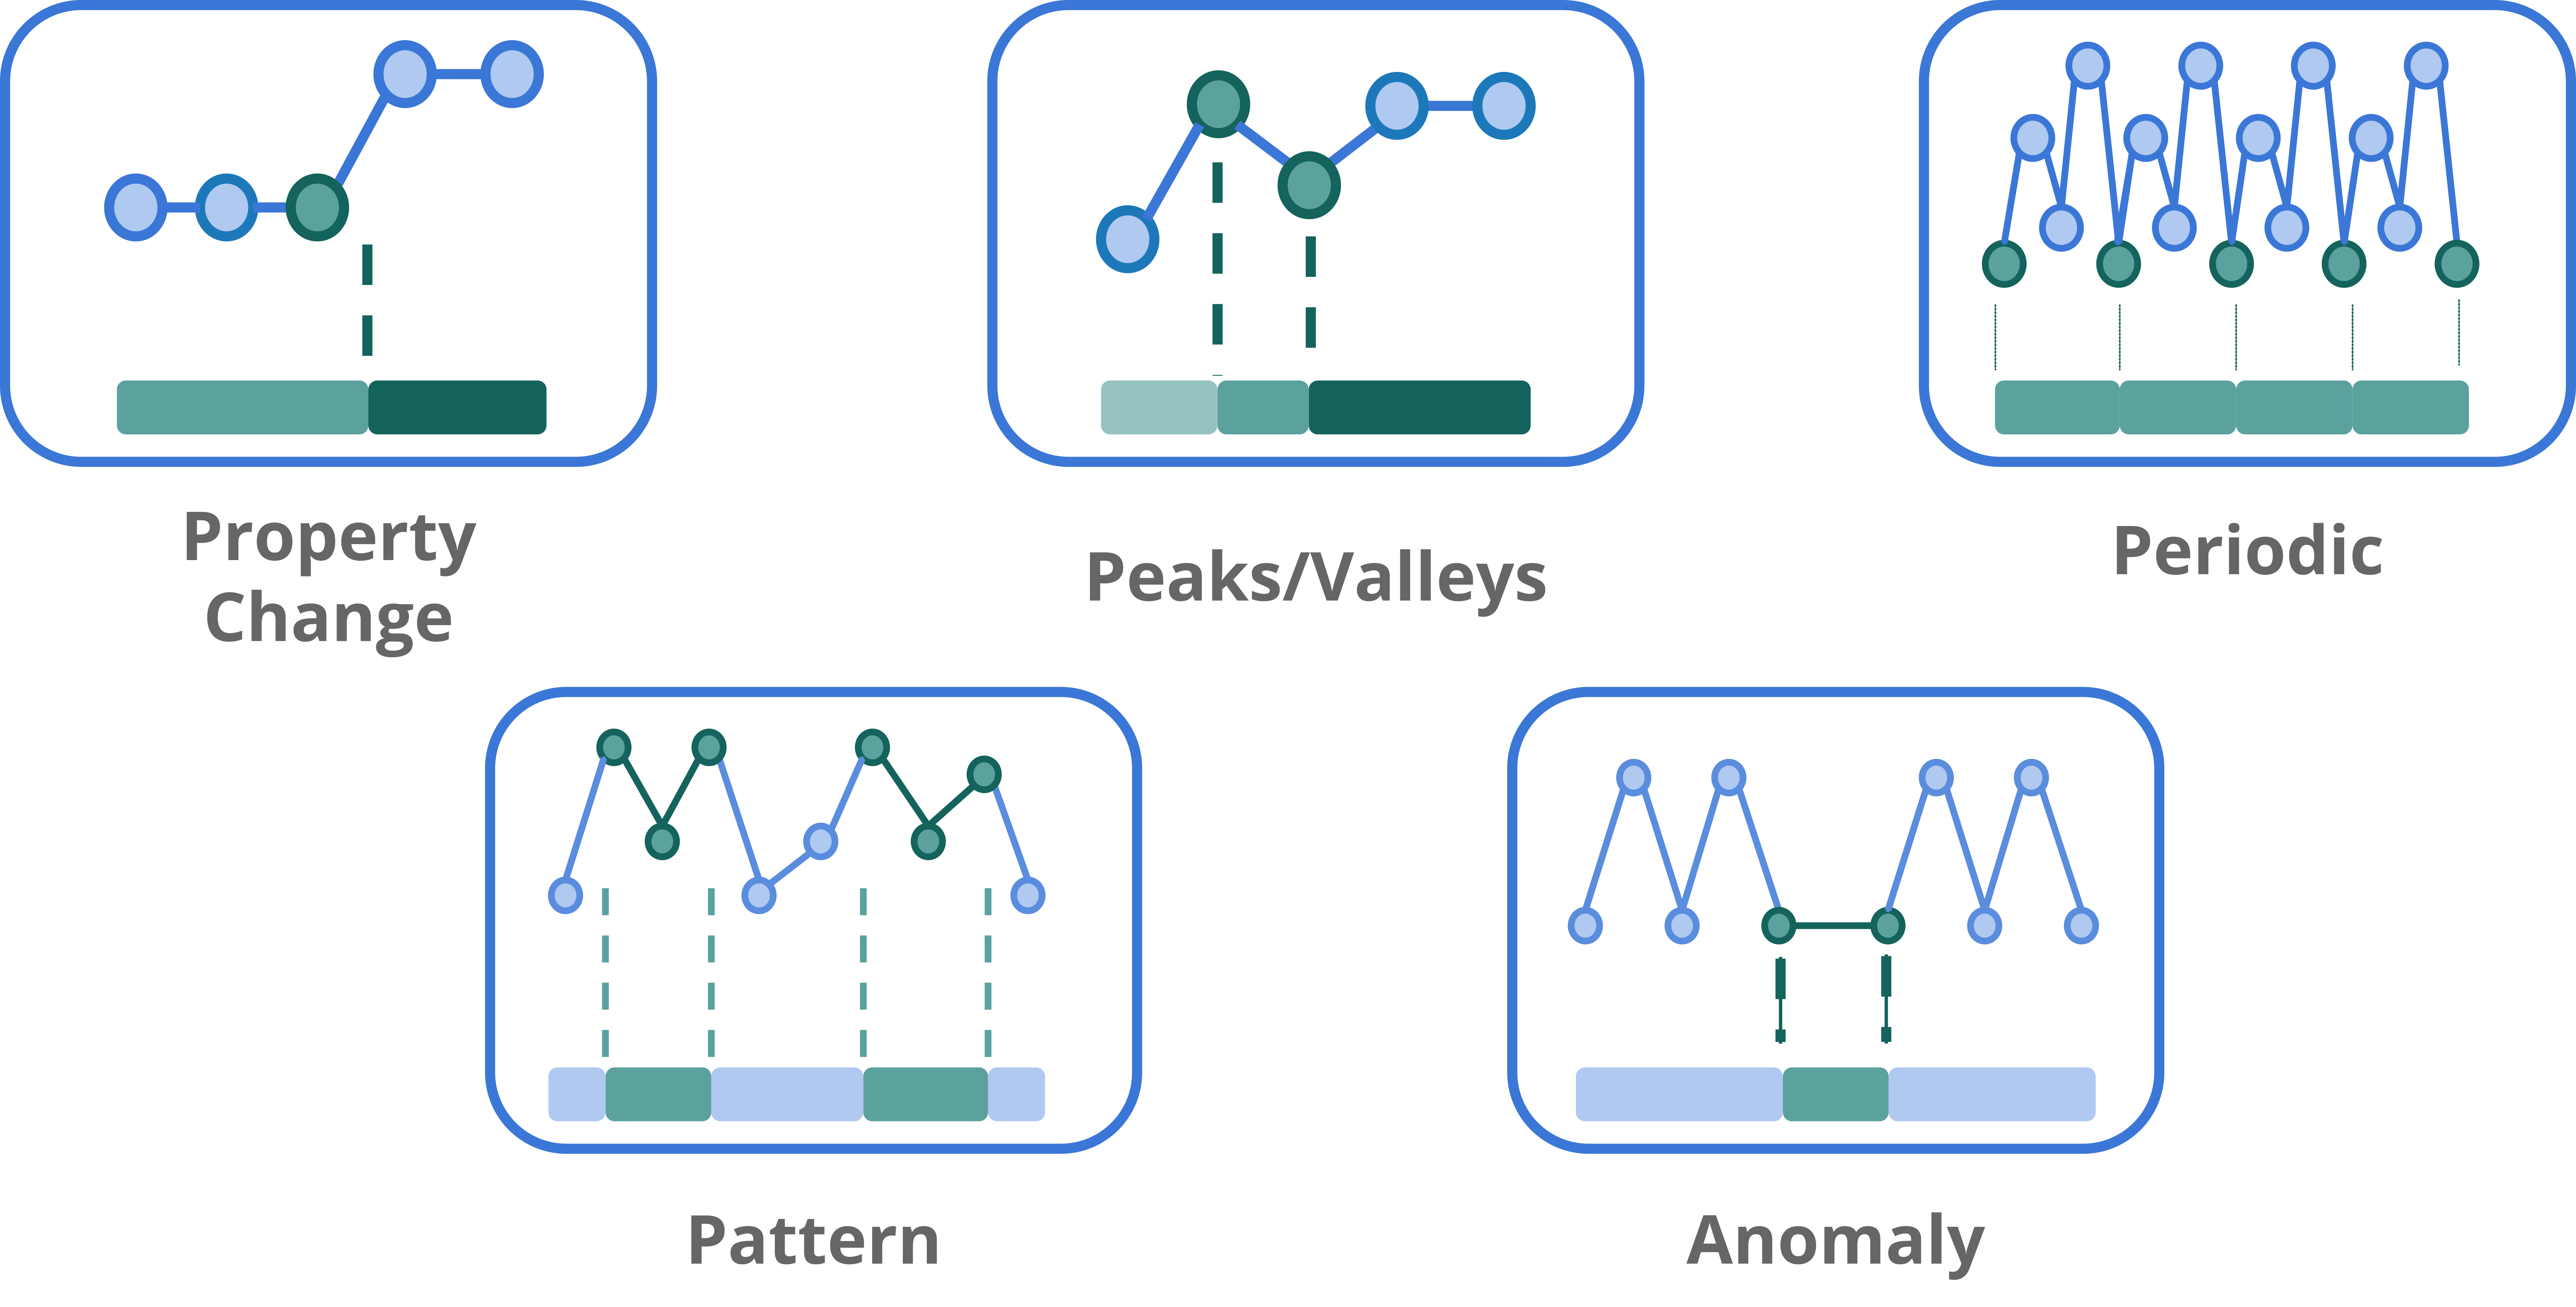
\includegraphics[width=0.95\linewidth]{event_type.png}
%	\label{fig:event_type}
%	\caption{}
%\end{subfigure}
%\caption{(a) Categories of search of events. In this case are shown Dimension, Window and Domain. (b) Examples of different type of events that can be considered significant in a time series.}
%\end{figure}


Figure \ref{fig:event_search} illustrates the search ranks of the problem formed by three layers:

\begin{itemize}
    \item \textbf{Dimensionality}: The search can be applied to one or multiple time series. In multidimensional space, some events can coincide in several time series, while others are specified on a particular dimension. For example, some gestures produce noticeable signals on only one dimension of the three-axis accelerometer.
    \item \textbf{Timescale}: \textit{Events}' occurrence can vary from different timescales. For example, when the signal being analysed is zoomed in from hour to minute scales, some events may disappear while new events may be detected.
    \item \textbf{Representation}: The searchable objects can be straightforwardly the temporal nature of time series or other representation, such as frequency or on other extracted features.
\end{itemize}

Besides the ranks mentioned above, the search procedure can be customized by context or target, which is highly related with the relevance given to an \textit{event} or a \textit{subsequence}. Types of events that are considered significant include:

\begin{itemize}
  \item \textbf{Property change}: The change of a property, such as a change in mean or frequency, or a set of properties is greater than a threshold, e.g., \textcolor{myblue}{low} to \textcolor{mygreen}{high} frequency - 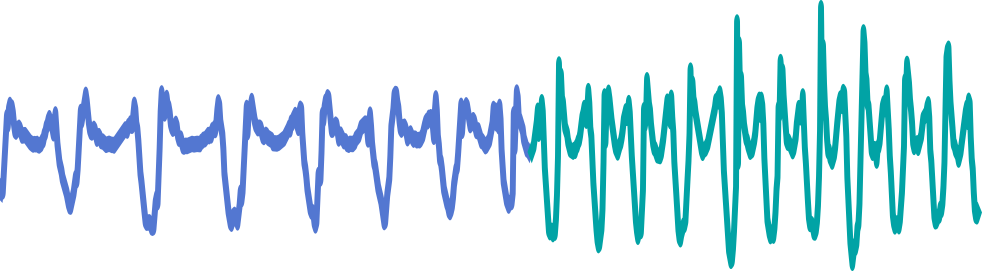
\includegraphics[height=2.5ex, valign=m]{walking_jogging.png}.
  \item \textbf{Peak/Valley}: Peaks and valleys can typically be associated with significant physical changes, e.g., \gls{ecg} \textcolor{mygreen2}{peaks} like 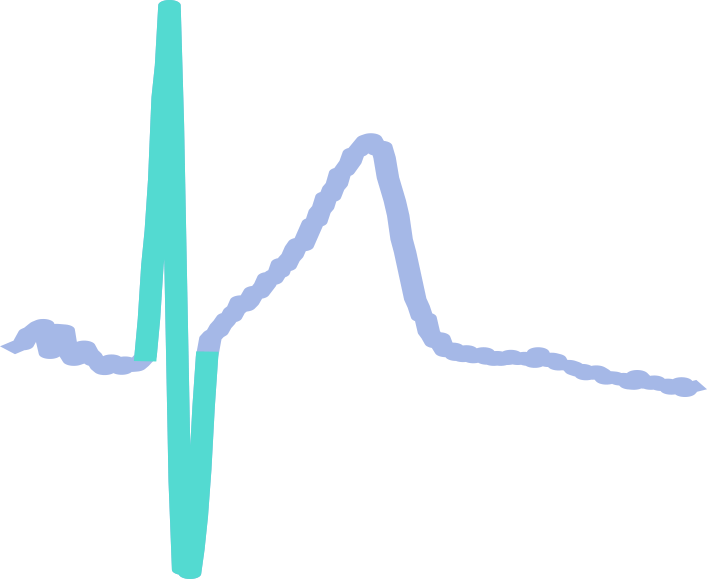
\includegraphics[height=3.5ex, valign=m]{high_peak_ecg.png}.
  \item \textbf{Periodicity}: The starting points of each period in a periodic signal are considered relevant, e.g., \gls{abp} periods like 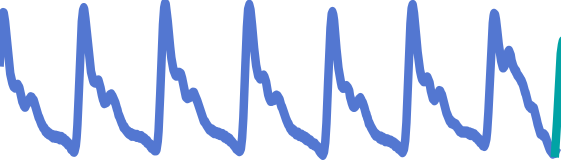
\includegraphics[height=2.5ex, valign=m]{bvp_segment.png}.
  \item \textbf{Recurrent pattern}: Re-occurrences of similar \textit{subsequences} with specific patterns should be of interest. Unlike \textit{periodicity}, \textit{recurrent} patterns do not have a temporal regularity.
  \item \textbf{Anomaly}: Highly dissimilar \textit{subsequences} with particular patterns are of the reference value, e.g., \textcolor{myred}{noise} in a clean signal 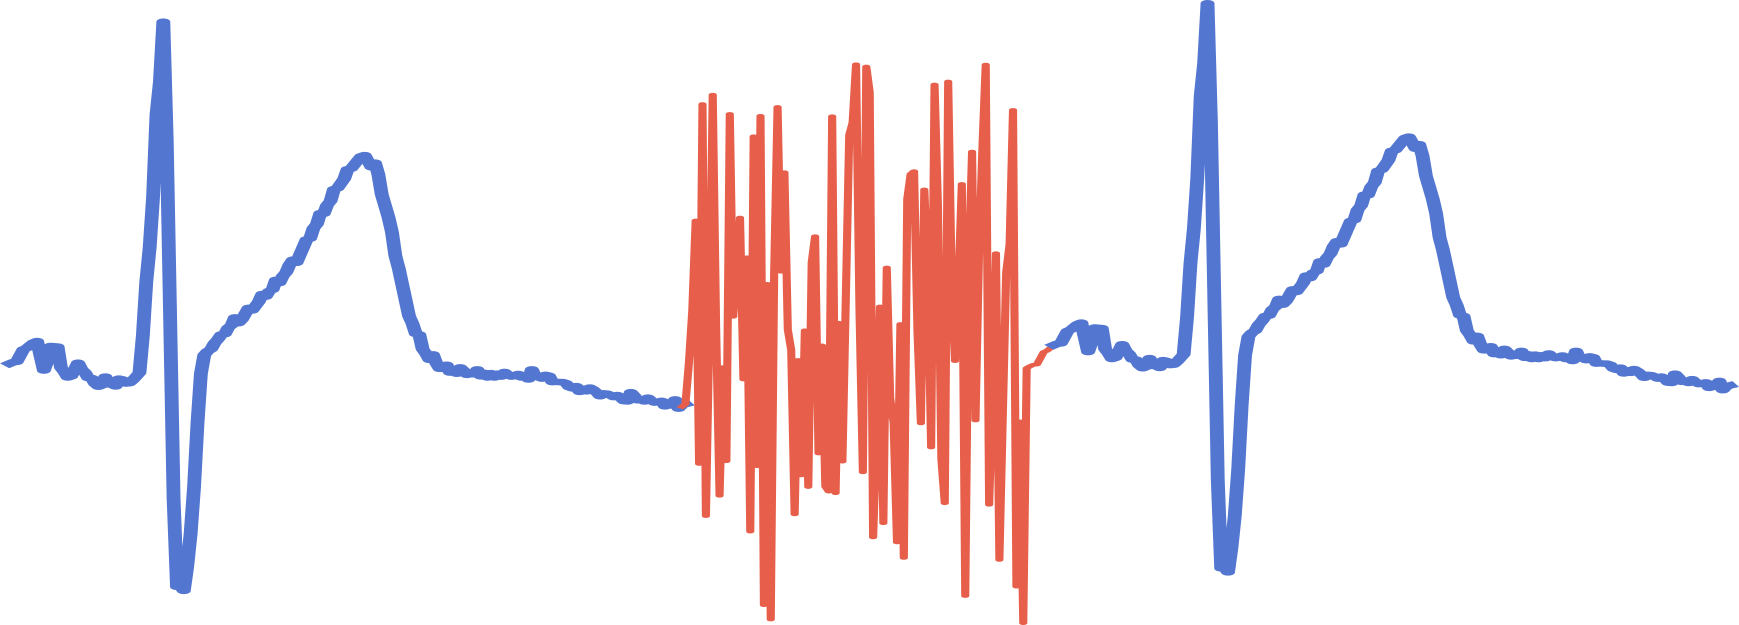
\includegraphics[height=3ex, valign=m]{ecg_noise_thumbnail.png}.
\end{itemize}

%Figures \ref{fig:event_search} and \ref{fig:event_type} are an illustrated summary of the two dimensions of the problem. Regarding the \textit{search} dimension, it is formed by three layers: \textit{(1) dimensionality}: the search can be made in one or multiple time series. In the multidimensional space, events can occur simultaneously in several time series, but other events can be specified for each of them (e.g. an accelerometer signal has 3 dimensions, but some gestures might be noticeable in only one of them); \textit{(2) time scale}: \textit{events} might occur in different time scales (e.g. when looking into a time series of 1 hour long, we might see some relevant events, but when looking for a \textit{subsequence} of 10 minutes (zooming-in), other events are revealed); \textit{(3) domain}: the search procedure might be made directly on the time series using time properties, a distance measure (e.g. \gls{ed}), or can be made on another representation level, such as the feature domain.
%
%In what regards the \textit{event} type, we show in Figure \ref{fig:event_type} examples of events that are considered significant in a time series: \textit{(1) Property change:} when the change of a property or set of properties is greater than a threshold, such as changes on the mean (FIND THUMBNAIL IMAGE) or frequency (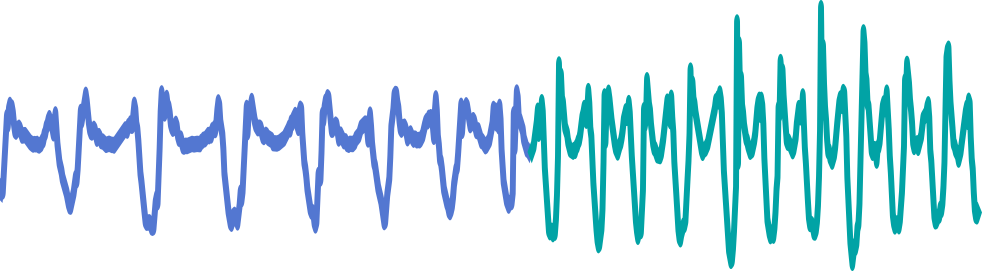
\includegraphics[height=3.5ex, valign=m]{walking_jogging.png}), \textit{(2) Peak/Valley}: peaks and valleys can typically be associated with significant physical changes (e.g. the peaks of an \gls{ecg} signal 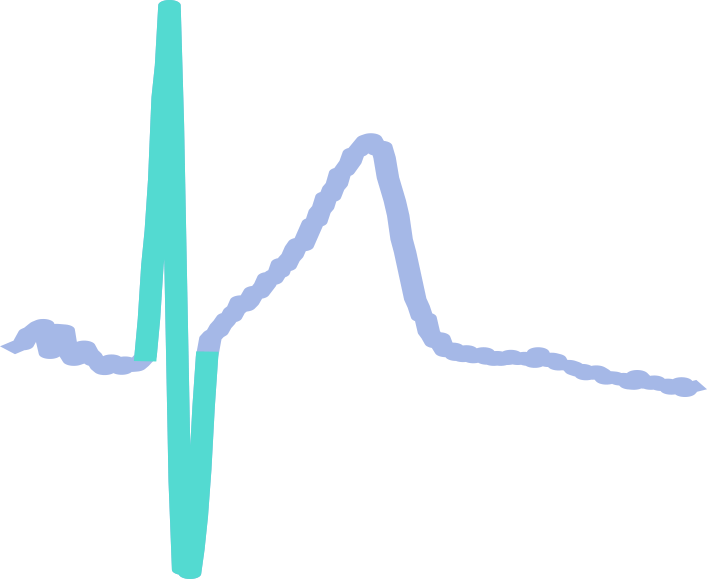
\includegraphics[height=3.5ex, valign=m]{high_peak_ecg.png}), \textit{(3) Periodicity}: if a signal is periodic, the moment each period starts is considered relevant (e.g. the cycles of a BVP signal 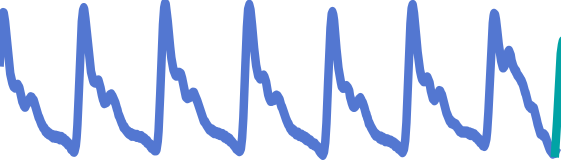
\includegraphics[height=2.5ex, valign=m]{bvp_segment.png}), \textit{(4) recurrent pattern}: re-occurrences of similar \textit{subsequences} with a certain shape or \textit{(5) anomaly}: very dissimilar \textit{subsequences} are relevant to indicate (e.g. noise in a clean signal 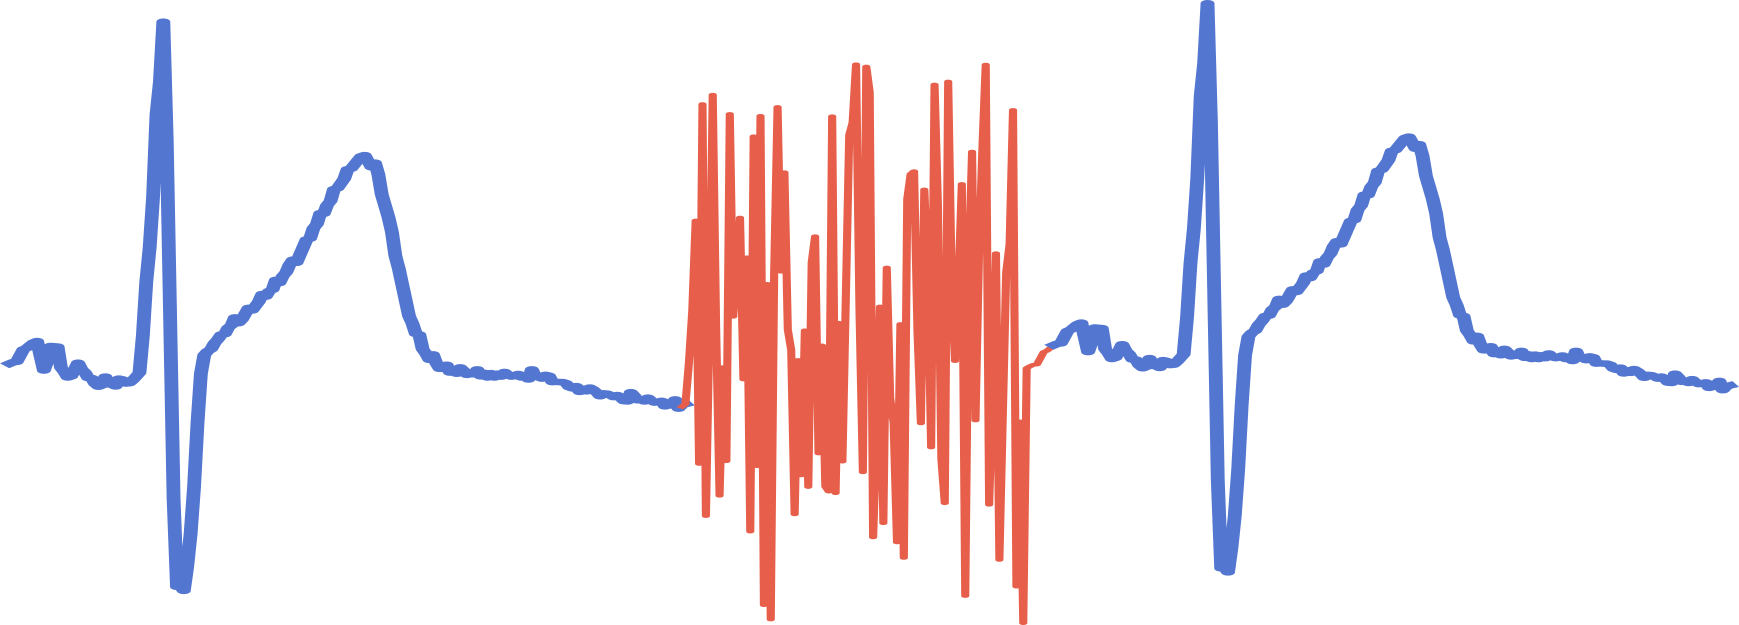
\includegraphics[height=3ex, valign=m]{ecg_noise_thumbnail.png}).

\subsection{Proposal}

In order to fill as many research gaps as possible, this study started by defining the search space, considering that if the time series is transformed in the feature space, any feature's change would be relevant. For instance, changes in the mean, standard deviation, frequency or other properties are all options worth searching for. By characterizing the signal into the feature space, we can explore changes in all feature representations. Additionally, an event should separate two different behaviours. The notion of \textit{difference} in time series can be associated with \textit{distance/similarity}, enabling finding segmentation points, recurrent patterns, anomalies, and periodic shapes.

Therefore, we propose an unsupervised methodology that searches for events (1) in uni and multidimensional space, (2) with a fixed timescale and potential multi-timescale application opportunities, and (3) on an \gls{ssm} computed by a feature space representation of the time series. The events to be searched are any changes in the \gls{ssm} related to a segmentation point and/or a periodic event.
\par
The proposed method's reliability for event detection will be evidenced by considerable experiments in various type-agnostic databanks of multiple time series domains and comparisons to the state-of-the-art methods. It should be highlighted that events in different datasets are extracted from the same information source, i.e., \gls{ssm}, which meanwhile provides insights into unsupervised automatic labelling.

    
%IMPORTANT
%Besides, at the feature level, we can very easily include the information of \textit{MTS}. The fact that features can be used for this purpose might help in targeting and fine-tuning the selection of features that work better for specific types of events or work domains (e.g. we might only be interested in changes related to the frequency and not mean fluctuations, therefore, frequency features should be chosen, making targeted event search).

%Tools: Annotation, Segmentation, One-click segmentation of periodic events, summarization, and profiling

\section{Building the SSM}

In this section, we explain the steps of the proposed method. The extraction of relevant events from time series starts by computing the \gls{ssm}. As explained in Section \ref{subsec:dist_matrix}, this matrix has relevant structural information to retrieve \textit{events}, namely \textit{blocks}, \textit{paths} and \textit{similarity profiles}. Figure \ref{fig:SSM_scheme} summarizes the steps involved in calculating the \gls{ssm}.

\begin{figure}
\centering
    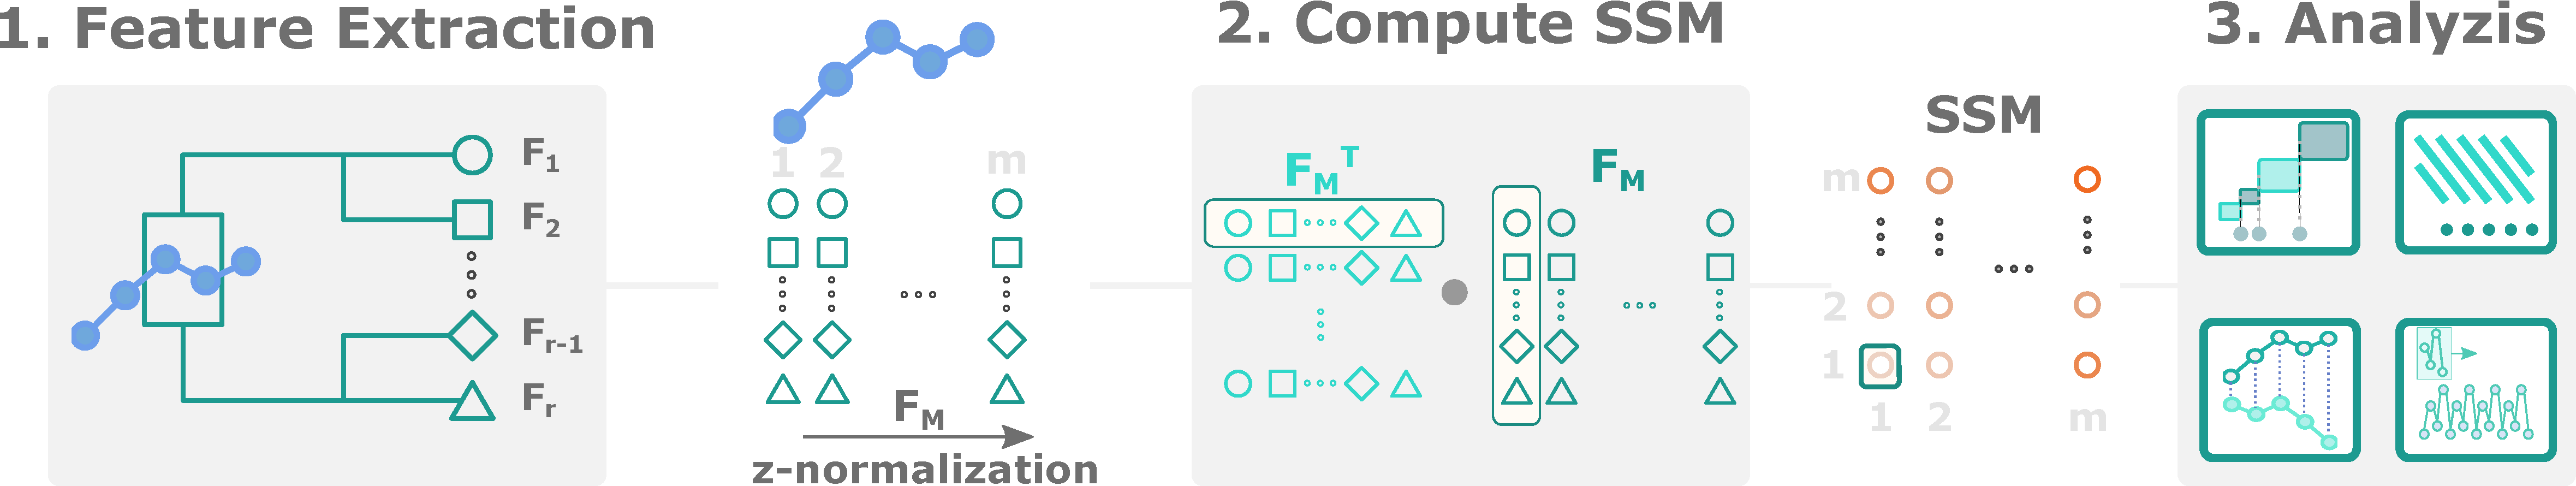
\includegraphics[width=\linewidth]{SSM_steps.pdf}
    \caption{Main process to reach the \gls{ssm}. The information needed to calculate the \gls{ssm} is the record and the input parameters: the window size ($w$) and the overlapping percentage ($o$). The first stage involves the feature extraction process, based on $w$ and $o$ values. Features are extracted on each subsequence $(sT_1, sT_2..., sT_N)$, being $N$ the total number of windows. From the first window ($sT_1$), are extracted features $(f1, f2..., f_K)$, being $K$ the number of features used. The feature number is also associated with a shape (circle, triangle, etc...). The features can be extracted on multivariate records, being $M$ the number of records used. Each feature is positioned as a row on the $F_M$ and the \gls{ssm} is computed from it.}
    \label{fig:SSM_scheme}
\end{figure}

\subsection{Feature Extraction}

The structural information present on the \gls{ssm} depends on the richness of the set of features into translating the changes and disruptions of the signal. Behavioral changes might be related to a variate set of features. As a feature may be sensitive to a type of change, the set of features should be diverse to identify a multivariate set of events and be agnostic to all types of signals. For this purpose, we used the available features from the \textit{TSFEL} \cite{barandas_tsfel_2020} Python library presented in the Feature Table \ref{tab:tsfel_featurelist} from Appendix \ref{app:tsfel}.
\par
The features are extracted with a moving window with size $w$, specified by the user, with an overlap of size $o$. These two parameters have a large influence on the results. The first defines the time scale at which features are extracted, therefore the wider the window, the more \textit{zoomed-out} will be the search. The second parameter defines the pixel-resolution of the resulting feature series, decreasing the amount of information (down-sampling) with a smaller overlap.
\par
The extracted features are grouped into a feature matrix ($F_{M}$), where the rows represent a feature series and the columns the corresponding \textit{subsequence}, described by all features. Features extracted from a multidimensional record are ordered in the $F_M$ as rows as well. The total number of rows can be, at maximum: $r \times k$, being $k$ the number of time series being analyzed and $r$ the number of features extracted, as illustrated in Figure \ref{fig:SSM_scheme}.
\par
Each feature extracted is z-normalized to guarantee that each feature series (rows of the feature matrix) has a more equal contribution in the description of the signal. Additionally, a second normalization is applied to the feature vector (columns of the feature matrix), which optimizes the calculation of the cosine distance between feature vectors by simply adding the dot product to calculate the \gls{ssm}. As an example of two simple features (mean and variance) and their normalized versions, we show Figure \ref{fig:features_normalized}.

\begin{figure}
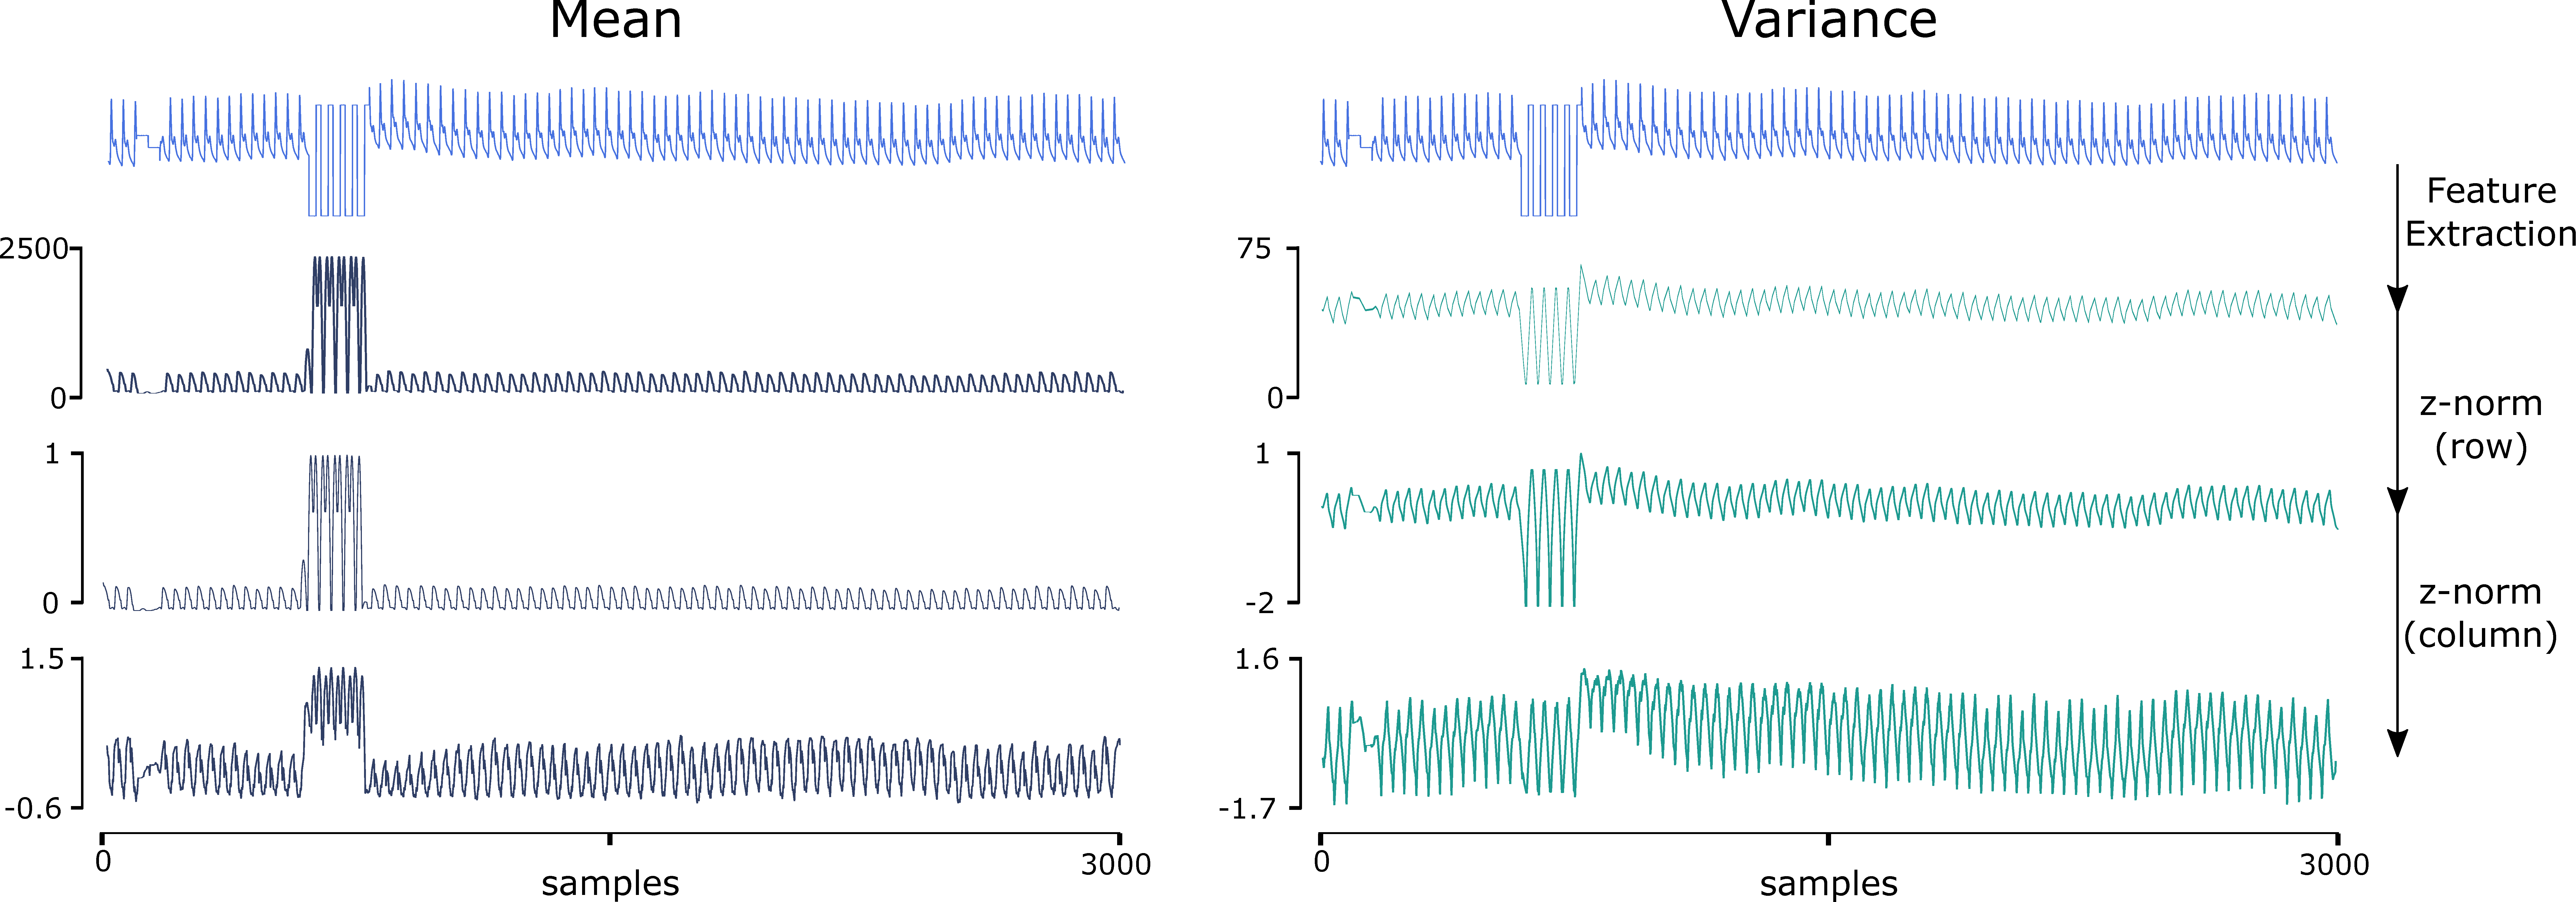
\includegraphics[width=\linewidth]{features_example.pdf}
\end{figure}


\subsection{Feature-based SSM}
\label{sec:the_ssm}

After grouping all the features extracted, the next stage is to apply a similarity measure to the feature space and compute the \gls{ssm}. This process consists in comparing each \textit{subsequence} with all the other \textit{subsequences} within the time series record. Since each column of the $F_M$ is the feature characterization of each \textit{subsequence} by the entire set of features, the comparison between segments is achieved by calculating the dot product between the z-normalized transposed $F_{M}$ and itself:

\begin{equation}
    SSM = F^T_M F_M
\end{equation}

The dot product gives a similarity score based on the feature values of each \textit{subsequence}. Cells of the \gls{ssm} with higher similarity scores indicate that the corresponding \textit{subsequences} have similar feature values \cite{audiolabs1, audiolabs2}. As a result, the \gls{ssm} provides rich visual information, highlighting structures, such as blocks and paths, that describe the signal's morphological behavior over time and its structure.

\begin{figure}
    \centering
    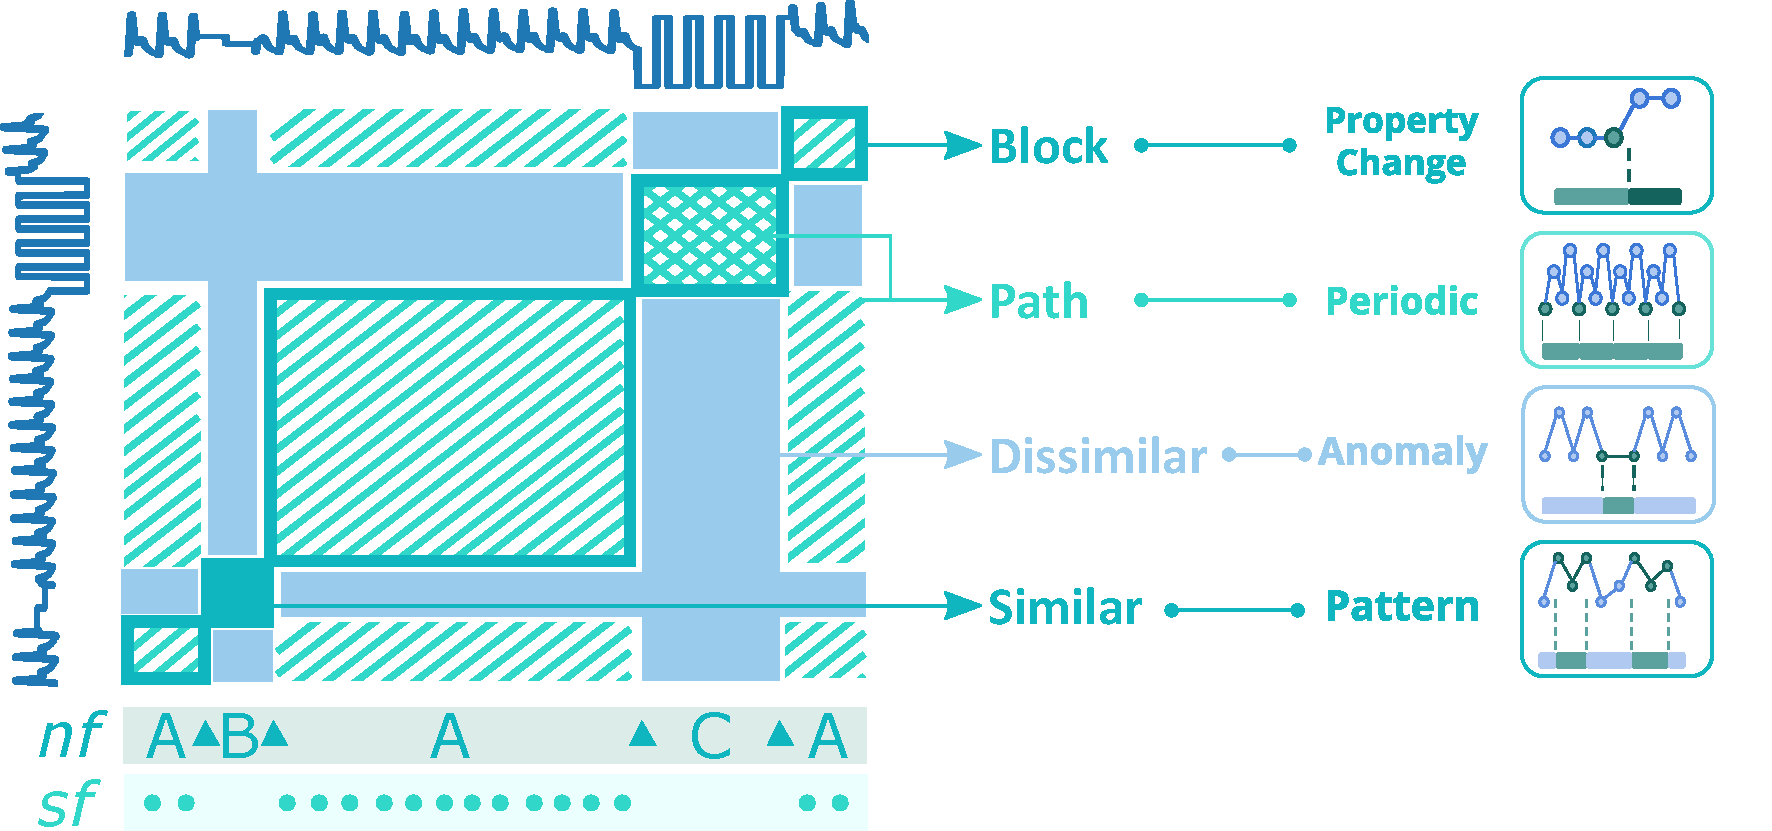
\includegraphics[width=\linewidth]{SSM_example.pdf}
    \caption{Description of informative structures of the \gls{ssm} of a \gls{abp} signal. We show a simplified view with highlights on the relevant structures. The record has 4 main structures: A - homogeneous segment, which corresponds to the \gls{abp} periodic signal; B - a homogeneous segment of missed data; C - homogeneous segment with a detachment of the sensor. The boxes highlight homogeneous behavior while the paths highlight periodicity in the segment. Segment C has a cross-pattern, which indicates periodicity and symmetry. $nf$ and $sf$ represent the novelty function and similarity function, respectively}. 
    \label{fig:ssm_description}
\end{figure}

In Figure \ref{fig:ssm_description}, the main structures are illustrated and highlighted in an example of an \textit{\gls{ssm}} \cite{audiolabs1} computed from an \gls{abp} signal. As mentioned in Chapter \ref{cha:methods1}, the main structures are \textit{blocks} and \textit{paths}. Our proposed method takes advantage of these main structures to extract the desired information.
\par
\textit{Paths} show recurrence of patterns, which is an indication of matching the morphology between corresponding \textit{subsequences}. The example highlights circles in the \textit{sf} layer, indicating when the paths start. In \textit{block} "C" are also visible \textit{cross-paths}, meaning that the \textit{subsequences} are periodic and symmetric.
\par
Differently, \textit{blocks} are square-shaped structures that indicate homogeneous areas of the \gls{ssm}, which translate as constant behavior in the time series. The change between block structures along the main diagonal indicates a relevant change in morphology and behavior in the time series. In Figure \ref{fig:ssm_description}, the \gls{ssm} is segmented into several blocks on layer \textit{nf}. The triangular shapes indicate the change points that separate blocks "A", "B", and "C". Besides \textit{paths} and \textit{blocks}, the \gls{ssm} provides similarity measures between \textit{subsequences}, which can be used to highlight (dis)similar segments, such as anomalies or highlight very similar \textit{subsequences}, such as motifs or cycles.
\par
Several strategies were applied on the \gls{ssm} to extract the mentioned information. Further are explained the approaches used.

\section{Information Retrieval}

The \gls{ssm} is a powerful visual tool \textit{per se}, highlighting relevant information that could be missed if looking at the raw time series. However, being the information on the \gls{ssm}, it should be possible to retrieve it automatically. As presented in Figure \ref{fig:info_retrieval_topics}, here are explained 4 approaches for information retrieval on the \gls{ssm}, namely (1) novelty search (\textit{block} transitions), (2) periodic search of patterns (\textit{paths}), (3) similarity profiles (how similar are the \textit{subsequences}) and (4) how to use a query from the \gls{ssm} to search for specific \textit{subsequences}. 


\subsection{Novelty Search}

The search for \textit{novelty} is inspired by a method used in musical structure analysis and presented by \textit{Foote et al.} \cite{foote2000}. The process involves searching for transitions between \textit{blocks} using a moving checkerboard square matrix. The result is a 1 dimensional function designated \textit{novelty function} - \textit{nova}.
\par
As shown in Figure \ref{fig:kernel_description}, block transitions along the diagonal are represented by a checkerboard pattern. Detecting such patterns can be made by correlating a standard checkerboard matrix with the diagonal of the \gls{ssm}. For this, a sliding squared matrix, designated \textit{kernel}, is used. As illustrated in Figure \ref{fig:kernel_shape}, the kernel has a checkerboard pattern and is combined with a Gaussian function to add a smoothing factor. The kernel, $K_N$, is a combination of two different square matrices: $K_H$ and $K_C$. The first is responsible for identifying the homogeneity of the \gls{ssm} on each side of the center point along the diagonal. The higher the homogeneity, the higher will be the values in these sections. The latter measures the level of cross-similarity, returning higher values in cases of high cross-similarity. Therefore, when sliding the kernel $K_N$ along the diagonal, a higher correlation value will be returned when it reaches a segment of the \gls{ssm} with a similar checkerboard pattern. The result is the mentioned $nova$ \cite{Dannenberg2008, fmp1, fmp2}.

\begin{figure}
    \centering
    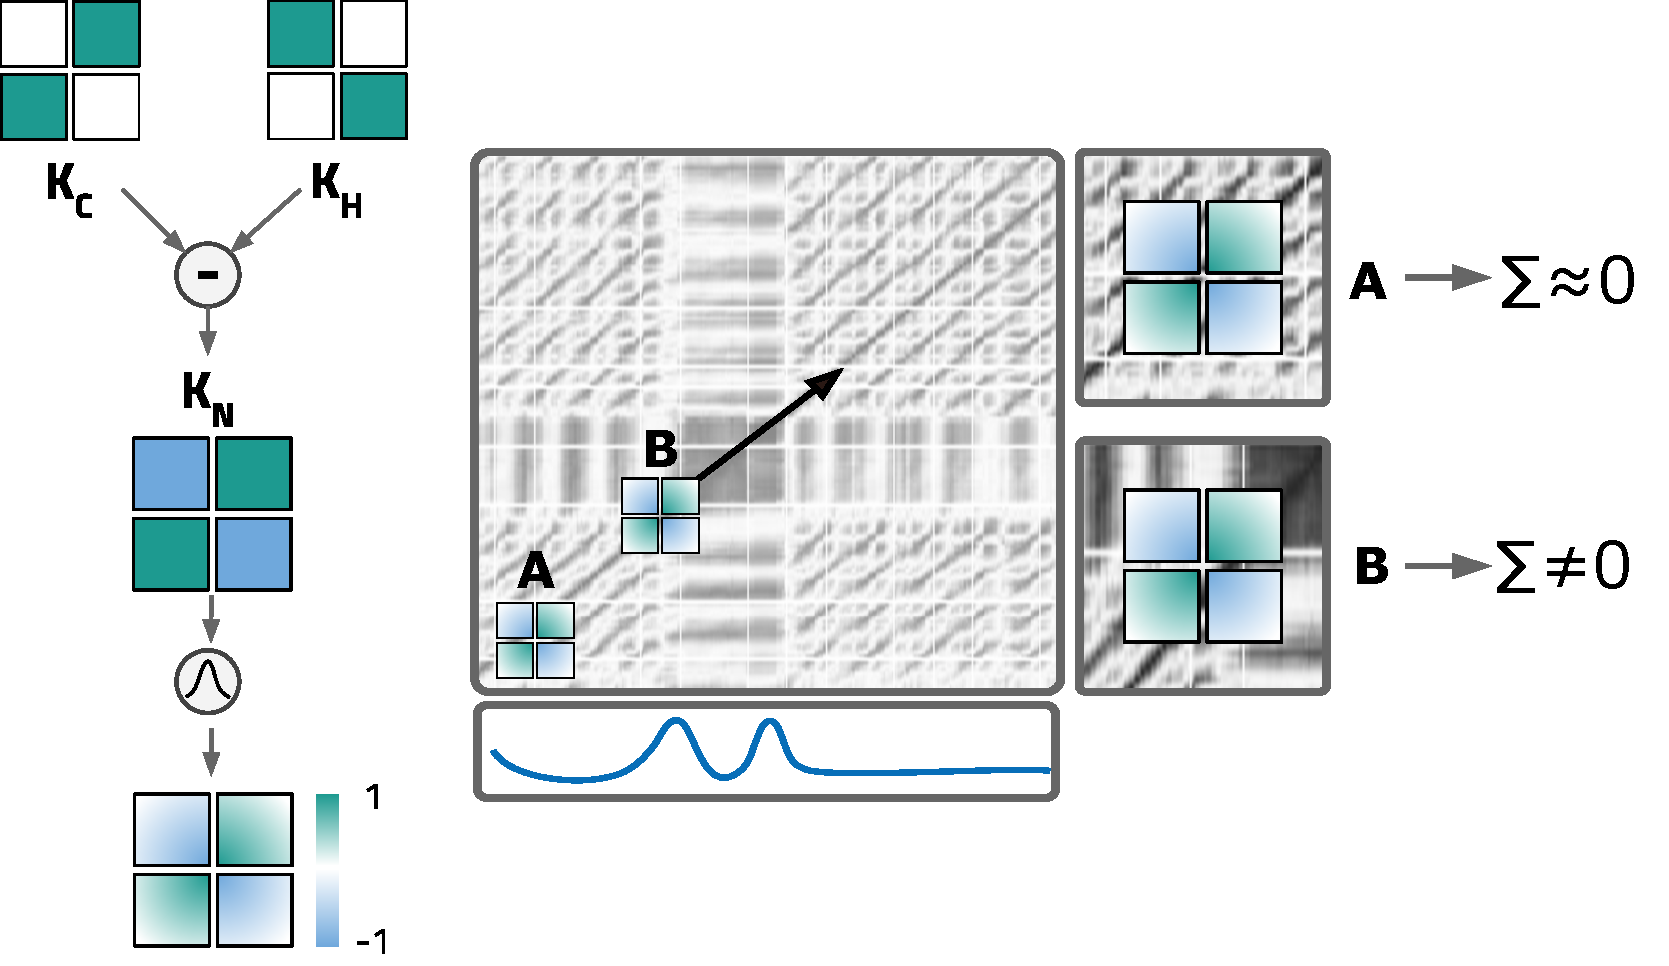
\includegraphics[width=\linewidth]{kernel_sliding.pdf}
    \caption{(left) Description of the matrix (kernel) used to compute the \textit{novelty function}. The checkerboard pattern is achieved by combining kernel $K_H$ - measure of homogeneity; and $K_C$ - measure of cross-similarity. The resulting kernel ($K_N$) is combined with a Gaussian function to generate $K_G$. The Figure is based on the works of \textit{Mueller et al.} \cite{fmp1, fmp2}; (right) The process to compute the novelty function is described. Kernel $K_G$ is slided along the diagonal of the \gls{ssm} to compute the \textit{novelty function} presented as the bottom sub-plot. Positions A and B show the effect of block transitions on the \textit{novelty function}. Figure based on the works of \cite{Dannenberg2008, fmp1, fmp2}.}
    \label{fig:kernel_description}
\end{figure}

As shown in Figure \ref{fig:kernel_description} (left), the kernel in position \textbf{A}, which is placed in an area of high homogeneity, returns a value close to $0$ when summing the product between it and the section of the \gls{ssm} it overlaps. On the other end, in position \textbf{B}, the kernel reaches a segment with low cross-similarity and high diagonal similarity, which results in high correlation values with a checkerboard pattern. The \textit{nova} is high in these transition segments \cite{Dannenberg2008, fmp1, fmp2}.
\par
Each section of the kernel has the same size, \textit{L}, being the total kernel size configured by $D = 2 \times L + 1$, with $L \in \mathbb{N}$ . The kernel has an odd size to adapt zero values in centered points. It also has total size D $\times$ D, being $K_{N}$ defined by the following function \cite{fmp1, fmp2}:

\begin{equation}
        K_N(i,j)  = \sign(a_i) \cdot \sign(b_j)
\end{equation}

being $a,b\in[-L:L]$ and $\sign$ representing the sign function, which indicates the sign of the value (1, 0 or -1). A radially symmetric Gaussian function is used to smooth the Kernel, with the following equation \cite{fmp1, fmp2}:

\begin{equation}
    \phi(p,u) = \exp(-\frac{1}{2L\sigma^2}(p^2 + u^2))
\end{equation}

being $\sigma$ the standard deviation, equal for both $x$ and $y$ dimensions of the matrix, $L$ the size of each kernel's section, and $p$ and $u$ the position in the $x$ and $y$ dimensions, respectively. The final kernel is computed by point-wise multiplication with the Gaussian function:

\begin{equation}
    K_{G} = \phi \cdot K_{N}    
\end{equation}

The \textit{nova} is calculated by correlating the kernel with the diagonal of the matrix:

\begin{equation}
    nova(m) = \sum^{2L+1}_{i,j=0} K_{G}(a_i,b_j)SSM(m+a_i, m+b_j)
\end{equation}

being the sample of the novelty function $m \in [0-N]$ and $a, b \in [-L:L]$. The change point events are represented by local maxima (peaks) in \textit{nova}, which can be detected by standard peak finding strategies.

\subsection{Periodic Search}

As aforementioned, \textit{paths} indicate the presence of similarity and reoccurring patterns can be visualized on the \gls{ssm}. The moment in time the \textit{paths} start indicates the position at which the period of the pattern begins. In order to find the periodicity, we compute the similarity function, $s_f$, which is calculated by summing the values of the $\gls{ssm}$ column-wise (either column-wise or row-wise would work, since the matrix is symmetric), being each element of the $sf$ calculated by:

\begin{equation}
sf(x) = \sum_{i=0}^{m}{SSM_{ix}}
\end{equation}

\noindent where \textit{i} is the column position for the sum, $sf_{j}$ the sample of the function at position \textit{j} and \textit{m} the size of one of the dimensions of the \gls{ssm}, which is equal to the feature-series size. As segments with similar morphology will be similarly described by the extracted features, the columns will have a similar representation, hence a similar value on the \textit{sf}. In cases where the time series is periodic, the similarity function will enhance this behavior. The identification of events related to the periodicity of a time series is then possible by searching for local minima (valleys) on the similarity function.
\par
Although not validated in this work, we highlight that the similarity function can have an additional purpose. Considering that each sample of the $sf$ is an average similarity of a subsequence to all other subsequences, it is possible to find \textit{anomalies}. If we define \textit{anomaly} as a subsequence highly unique and different from all the rest of the time series, then the average similarity to all the other subsequences should be low, meaning that a sample of the $sf$ that represents an anomaly should have a lower value. 

\subsection{Similarity Profiles}

The main elements, \textit{blocks} and \textit{paths}, are essential sources of information for the segmentation of the time series. Besides these, the \gls{ssm} also provides the pairwise similarity values between all \textit{subsequences} of the time series. This is an important measure that gives an understanding of how close together are each \textit{subsequence} and can be used to cluster them or find either \textit{motifs} or \textit{discords}. In order to use the similarity values of the \gls{ssm} to compare \textit{subsequences} we can use the \textit{similarity profiles}. 
\par
A similarity profile, such as a distance profile explained in Section \ref{subsec:matrixprofile}, represents the similarity values of a \textit{subsequence} to all the other \textit{subsequences}. This simply represents one column/row of the \gls{ssm}. An example of a \textit{similarity profile} from the \gls{abp} signal is presented on Figure \ref{fig:abp_sim_profile}. We can find maximum values where the signal is more similar to the \textit{subsequence} from which the profile is being computed. We find that this profile can be used to compare \textit{subsequences} but also entire segments of the signal. Take for instance all three segments $A$ highlighted on Figure \ref{fig:SSM_scheme}. Although having different size, their profile is highly similar. 
\par
Although the comparison between segments could be made by directly using the region of the \gls{ssm} delimited by both \textit{subsequences}, we find that a stronger measure is to compare how much each of the two segments is similar/different based on their similarity/distance to all the other \textit{subsequences} of the time series. For this, a \textit{similarity profile} ($P_s(c)$) of a segment is computed as the column(row)-wise average similarity values of the region of the \gls{ssm} delimited by the segment being profiled, with size $l$, and all the other \textit{subsequences} of the time series, with size $m$:

\begin{equation}
P_s(c) = \frac{\Sigma_{i=0}^l SSM(i, c)}{l}
\end{equation}

The \textit{similarity profile} is computed column(row)-wise, being each column(row) $c(r)$ the average similarity value between the reference segment and the segment corresponding to $c$. The reasoning is that similar segments should have closer \textit{similarity profiles}. Since the profiles have the same size, these can then be compared with the \gls{ed} and clustered based on these distance values. This process can be specially valuable to cluster the segments previously extracted with the \textit{nova} and \textit{similarity} functions.

\begin{figure}
\centering
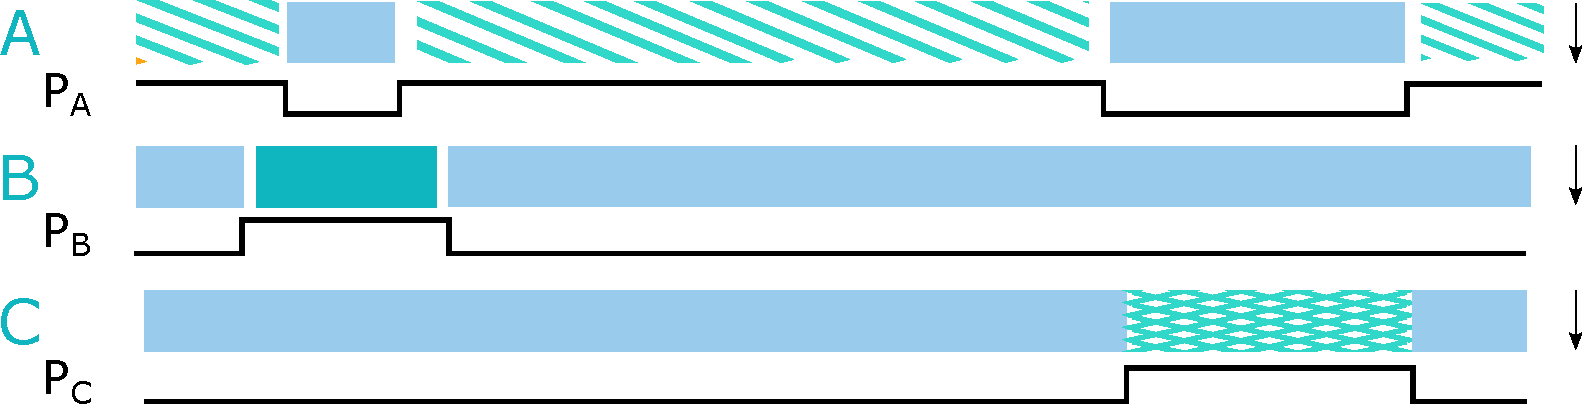
\includegraphics[width=\linewidth]{profiles.pdf}
\caption{Profiles computed for each segment of the example signal used in Figure \ref{fig:ssm_description}.}
\end{figure}

A general example of applying this process to the segmented time series based on the \textit{nova} function is showed in Figure \ref{fig:profiles}. Each segment category (A, B and C) extracted from the \gls{ssm} of Figure \ref{fig:ssm_description} is computed into a profile ($P_A$, $P_B$ and $P_C$) by averaging column-wise. These \textit{similarity profiles}show how similar the segment is with all the other \textit{subsequences} of the time series. All segments A will have a similar $P_A$, while being very different from profiles $P_B$ and $P_C$. 

\subsection{Query Search}
\label{subsec:query_based}

The mentioned similarity profiles are also useful to search for specific repetitions of a query from the time series. The process follows the traditional methods of template-based search methods explained in Chapter \ref{subsec:query_based_search), but instead of doing the process directly on the time series, it is performed on the \gls{ssm}. The search procedure works by sliding the smaller column window (the example selected on the time series) along the \gls{ssm}, one sample at a time. The distance, $D$, between the example and the segment it slides over is calculated through the sum of absolute differences:

\begin{equation}
    D(i) = \sum_{i=0}^{i=m}{\sqrt{(SSM(i) - SSM_t)^2}}
\end{equation}

where $SSM(i)$ is the segment of the \gls{ssm} over which the example, $SSM_t$, slides at moment $i$, up to the size of the \gls{ssm}. The resulting distance function has minimums at the position where the example is matched.


\section{Experimental Evaluation in Selected Use-cases}
\label{sec:use_cases_ssm}

After explaining the process to represent the time series into a feature-based similarity matrix and the methods used to retrieve information from it, we present selected use-cases from multiple domains to exemplify its universal usage.

\subsection{Use-Case 1 - Human Activity}

\begin{figure}
    \centering
    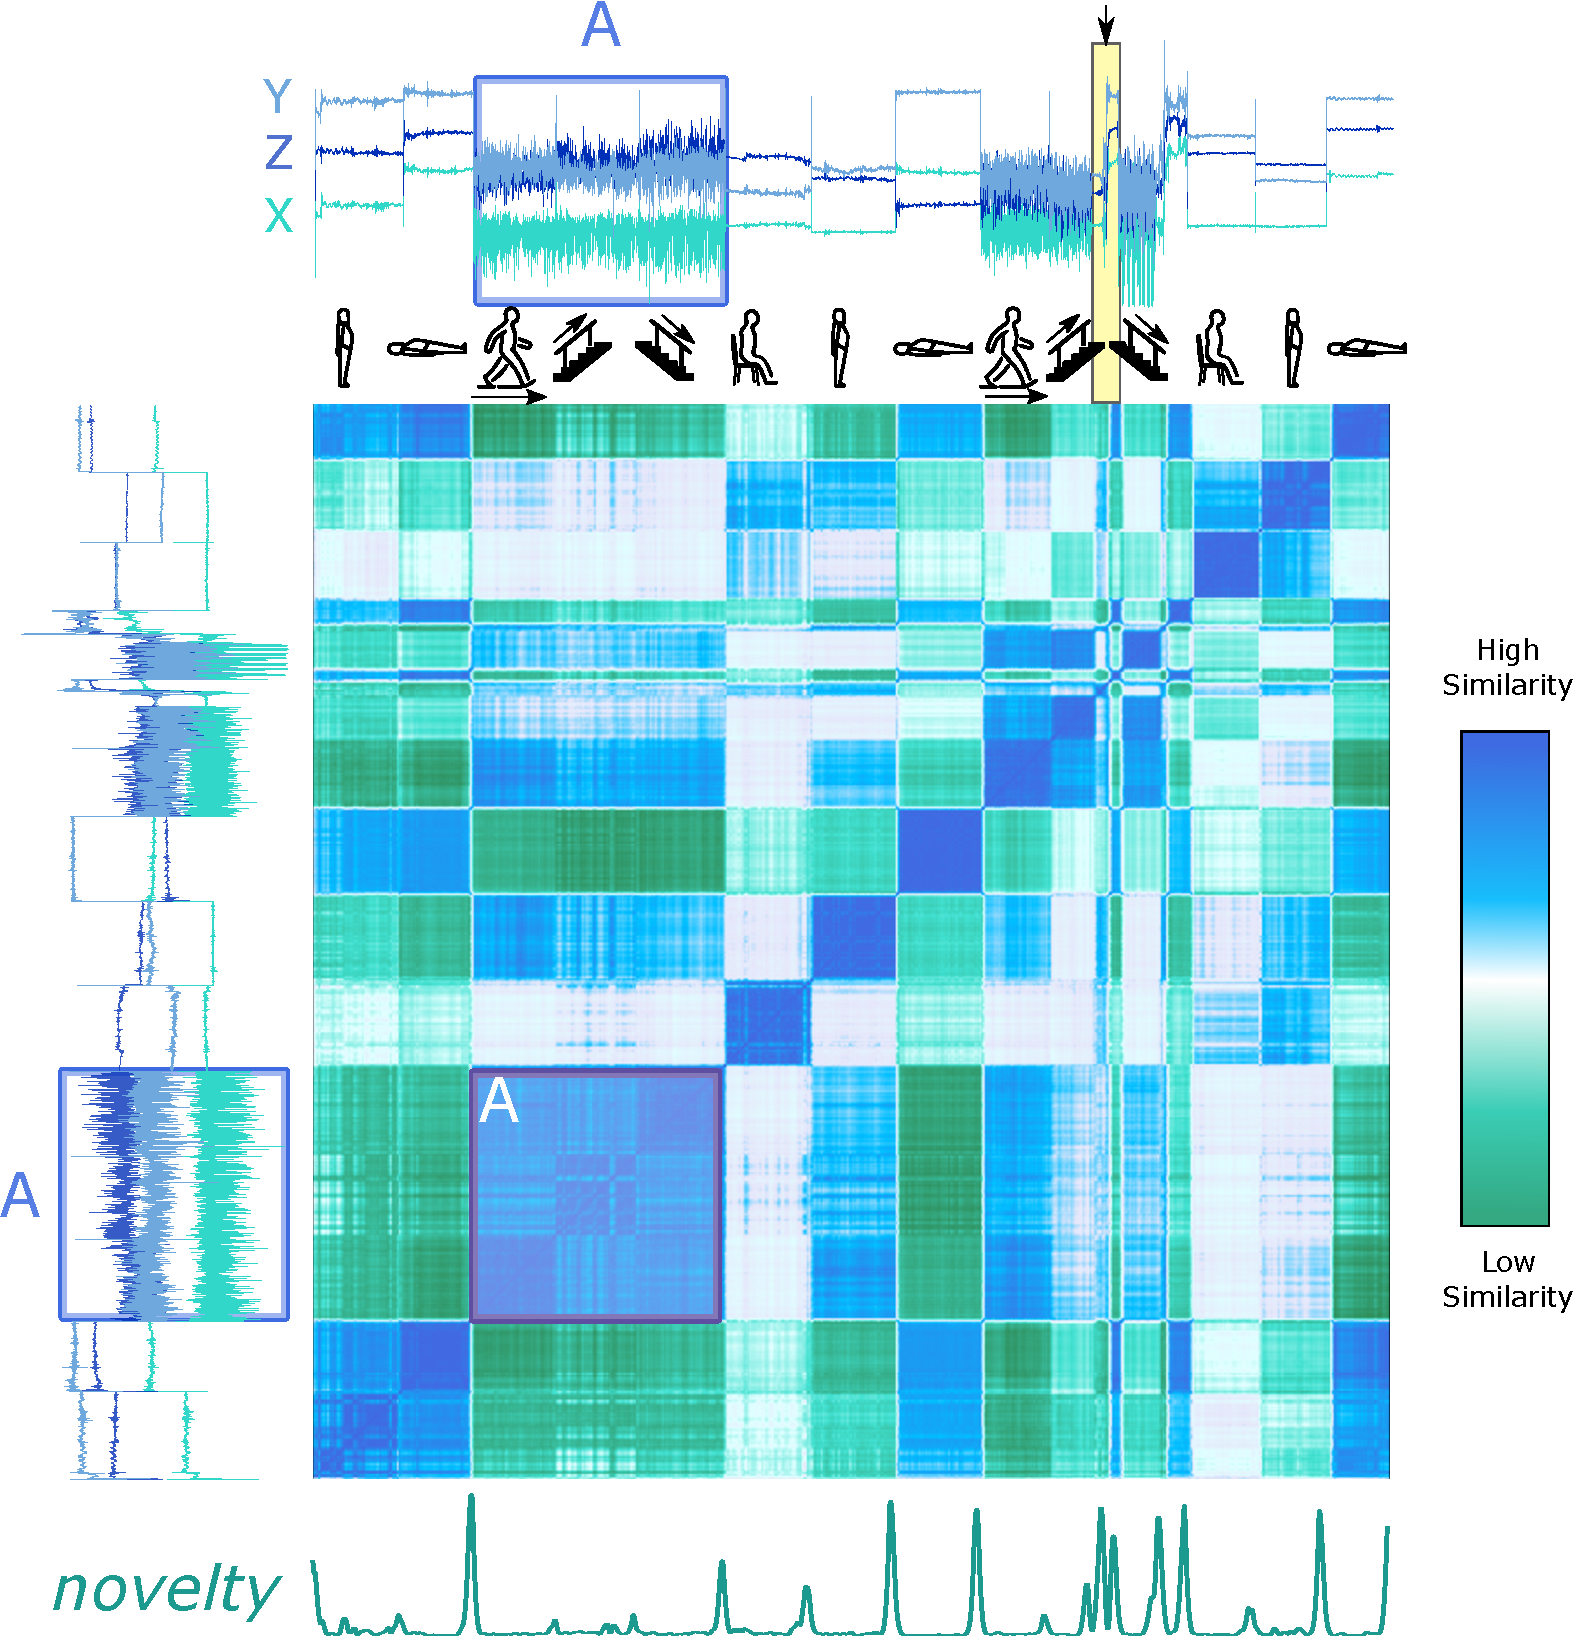
\includegraphics[width=\linewidth]{use_case1_HAR.pdf}
    \caption{Change point event detection strategy applied on the \gls{ssm} to search for change point events. The sequence of activities is presented as follows: $Sitting \xrightarrow[]{} Laying \xrightarrow[]{} Walking \xrightarrow[]{} Upstairs \xrightarrow[]{} Downstairs \xrightarrow[]{} Sitting \xrightarrow[]{} Standing \xrightarrow[]{} Laying \xrightarrow[]{} Walking \xrightarrow[]{} Upstairs$. The input variables used are $time_{scale}$=250 samples, $kernel_{size}$=45 samples, overlap=95\%}
    \label{fig:use_case1}
\end{figure}

The example presented in Figure \ref{fig:event_search_demonstration} shows the usage of the \gls{ssm} on a record of Dataset 2. In this example, the method was applied to all the 3-axis of the accelerometer data. All are shown and described with the sequence of activities as captioned in Figure \ref{fig:use_case1}.
\par
The \gls{ssm} was computed using a window size of 250 samples, and an overlap of 95 \%. The color \textit{blue} indicates segments with higher similarity. Along the diagonal, these blocks are visible and the events are estimated as the transition between these, highlighted by the \textit{nova} function. The kernel used for this detection had a size of 45 samples.
\par
In this example, we can identify that the detected change point events match the activity transitions. Although all transitions are visible on the novelty function, the ones that correspond to transitions between similar segments of activities are harder to find, namely the transitions between walking activities. This is plausible since the properties of these segments are similar and the morphological difference is not as significant as when shifting between dissimilar activities (e.g. between \textit{Laying} and \textit{Walking}).
\par
Any significant change in properties will be detected by the proposed method. As presented in Figure \ref{fig:event_search_dimension}, at the end of the time series, the period in which the subject was performing the \textit{Walking upstairs} activity is affected by other changes in the time series. These are significant and also correspond to \textit{block} transitions, which are also evident in the novelty function. The proposed strategy, being unsupervised, is sensitive to any change, as long as it is observed as a significant change in the signal's properties\\


\begin{figure}
    \centering
    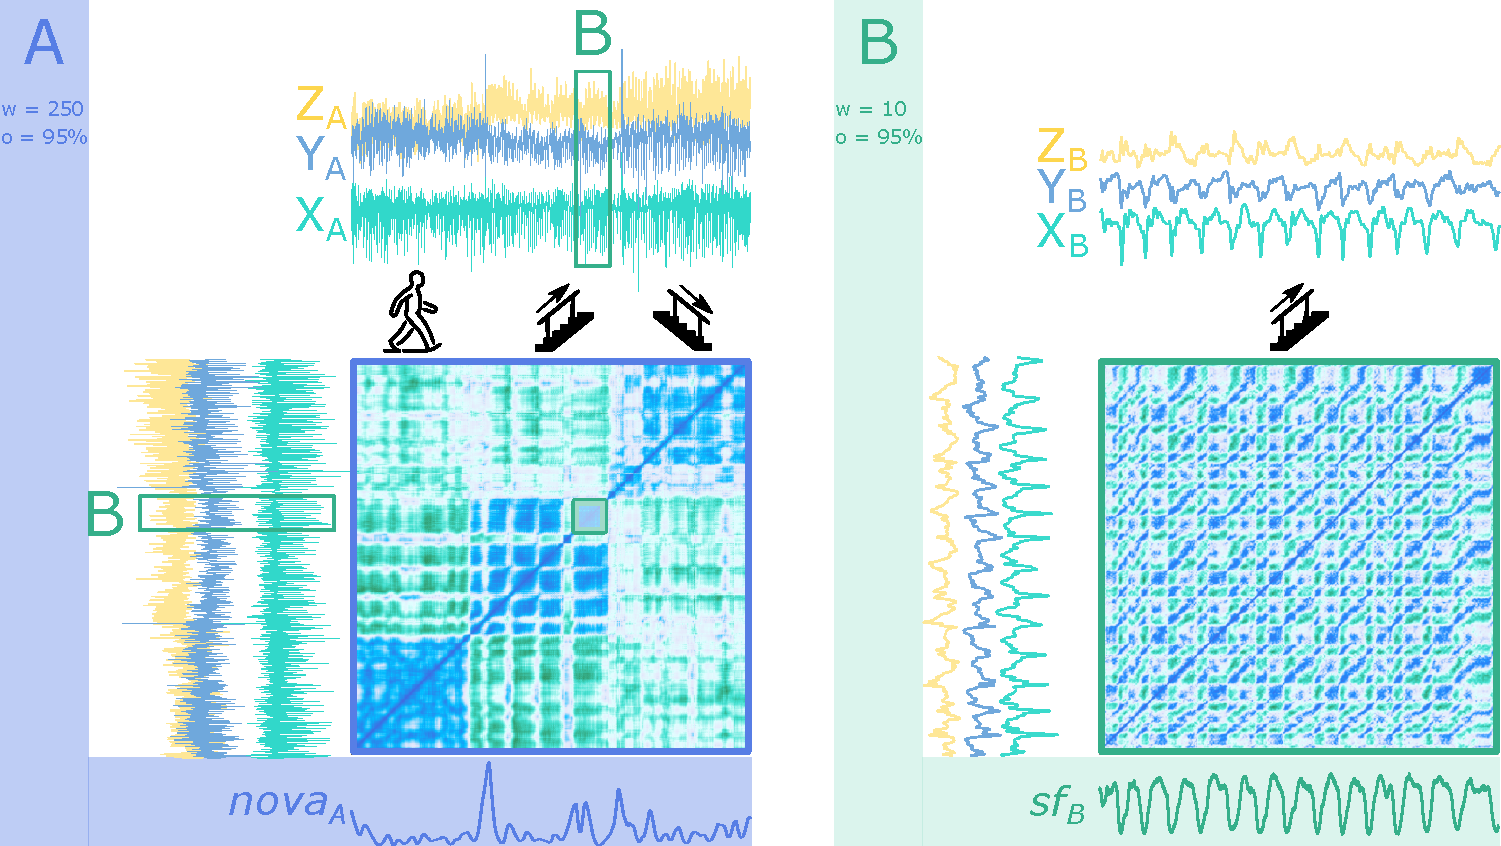
\includegraphics[width=\linewidth]{use_case1_HAR_zoom_in.pdf}
    \caption{\gls{abp} signal change point detection. The parameters used were a size of 5000 samples, with an overlap of 75\% and a kernel size of 25 samples.}
    \label{fig:example1_zoom}
\end{figure}

When \textit{zooming-in} the \gls{ssm} into segment \textit{A}, which shows transitions between walking behaviors, the checkerboard pattern that highlights change points are clearer and the three different walking patterns are easily segmented. The two major peaks in the corresponding \textit{nova} function are from these transitions, as presented in Figure \ref{fig:example1_zoom} (left). In addition, the reader might notice that the segments of the matrix related with \textit{walking in stairs} are also segmented into smaller \textit{blocks}. Although the information is not available in the dataset description, we strongly believe these are a flight of stairs.
\par
Considering that the signal is a walking behavior, the reader might question the fact that the periodicity of the walking pattern is not exhibited on the matrix. The reason is that the window size used to compute the \gls{ssm} of Figure \ref{fig:use_case1} is too large. If features are extracted with smaller window size, closer to the walking period, the \textit{paths} that indicate the recurrence of shapes are visible. Figure \ref{fig:example1_zoom} (right) shows the \gls{ssm} built from the segment \textit{B} of the original time series, with a window size of 10 samples and an overlap of 95 \%. The matrix shows the \textit{paths}, from which it is possible to extract the periods with the similarity function ($sf_B$).


\subsection{Use-Case 2 - Medical domain}

In the medical domain, there are several examples of structural information to retrieve. Some signals are periodic, such as the \gls{ecg}, the \gls{abp} or the \gls{resp} signals. When acquiring this type of data, several instances might reflect unexpected changes, either because of physiological responses, medical disorders or to the sensing process (such as noise from sensors, motion artifacts, sensor detachment, etc...). Here we show two examples of physiological changes in two periodic signals.

\begin{figure}
    \centering
    \includegraphics[width=0.9\linewidth]{5_abp_example_1.pdf}
    \caption{(a) \gls{abp} signal novelty search. The parameters used were a window size of 5000 samples, with an overlap of 95\% and a kernel size of 200 samples.}
    \label{fig:example2}
\end{figure}

The \gls{abp} signal can change due to postural changes. An experiment was conducted to study this effect and is available at Physionet \cite{tilt, PhysioNet}. Figure \ref{fig:example2} shows the process of segmenting the \gls{abp} signal based on postural changes, signaled with the ground truth (as the square signal). The change points are well perceived by the proposed strategy. The reader can notice that the shape of the \gls{abp} signal in each regime is very similar, being hard to notice by the human eye where it happened. This is an interesting result considering that it solely relies on the \gls{abp} signal for this detection. It is also important to point out that the periodicity of the signal is not visible on the matrix because the features were extracted with a window size of 5000 samples, which is much larger than the period length. However, we can perform this periodic segmentation if using a smaller window size (in this case of 250 samples). This process is illustrated on Figure \ref{fig:example2_periodic} where a segment of the original signal of Figure \ref{fig:example2} (the first 10000 samples) is computed into the \gls{ssm}. The resulting \textit{sf} shows the periods of the \gls{abp} signal quiet well.

\begin{figure}
    \centering
    \includegraphics[width=0.9\linewidth]{5_abp_example_2.pdf}
    \caption{\gls{abp} signal. It represents the first 10000 samples of the signal from Figure \ref{fig:example2}. The parameters used were a window size of 250 samples, with an overlap of 95\% and a kernel size of 200 samples.}
    \label{fig:example2_periodic}
\end{figure}

The \gls{ssm} of Figure \ref{fig:example2}.a also shows which segments are similar to each other. The blue colors of the matrix indicate high similarity and it is presenting that segments from the same posture are more similar. To show this we computed the similarity profiles of each segment (as if segmented by the \textit{nova} function) and show that the corresponding sections would be well clustered based on these profiles ($P_A = P_C$ and $P_B=P_D$). In the same way, the similarity profiles of the signal of Figure \ref{fig:example2_periodic} highlight also the similarity between segmented \textit{subsequences}. Profiles with a similar shape can be grouped together such that we can understand that $P_A=P_C=P_E=P_G$ and $P_B=P_D$.

\begin{figure}
    \centering
    \includegraphics[width=0.9\linewidth]{5_ecg_example.pdf}
    \caption{\gls{ecg} signal with a \textit{pulsus paradoxus} condition starting at the 10000th. The \gls{ssm} shows the two modes of the \gls{ecg}. Highlights of each mode are presented with the circle zoomed-in thumbnails. In more detailed are also shown segments A and B, which highlight an area where the \gls{ssm} indicates possible changes.}
    \label{fig:example2_3}
\end{figure}

The same happens on the \gls{ecg} signal from Figure \ref{fig:example2_3}.right. It displays the presence of a condition called \textit{pulsus paradoxus}, which is an exaggerated fall (>10 mmHg) in the patient's blood pressure during inspiration \cite{pulsusparadoxus2}. This also can occur when the patient's changes sleeping posture after a heart surgery\cite{eamonn_segmentation}. Detecting when these cases occur is an important task. The present example is a case of an \gls{ecg} that exhibits this condition.
Again, the reader can notice that the change point is hardly perceivable by the human eye, but the proposed strategy can clearly show the difference between both regimes.
\par
In addition to the novelty detection, it is visible on the first segment of the signal previous to the \textit{pulsus paradoxus} occurrence, that there are smaller segmentation points. Zooming into the signal (segment A), it is not clear what this can be, but zooming further into segment B makes it clear that there are minor changes on the \gls{ecg} due to additional noise on some segments. This method would be able to segment it to.

\subsection{Use-case 3 - Multidimensional}

\begin{figure}
    \centering
    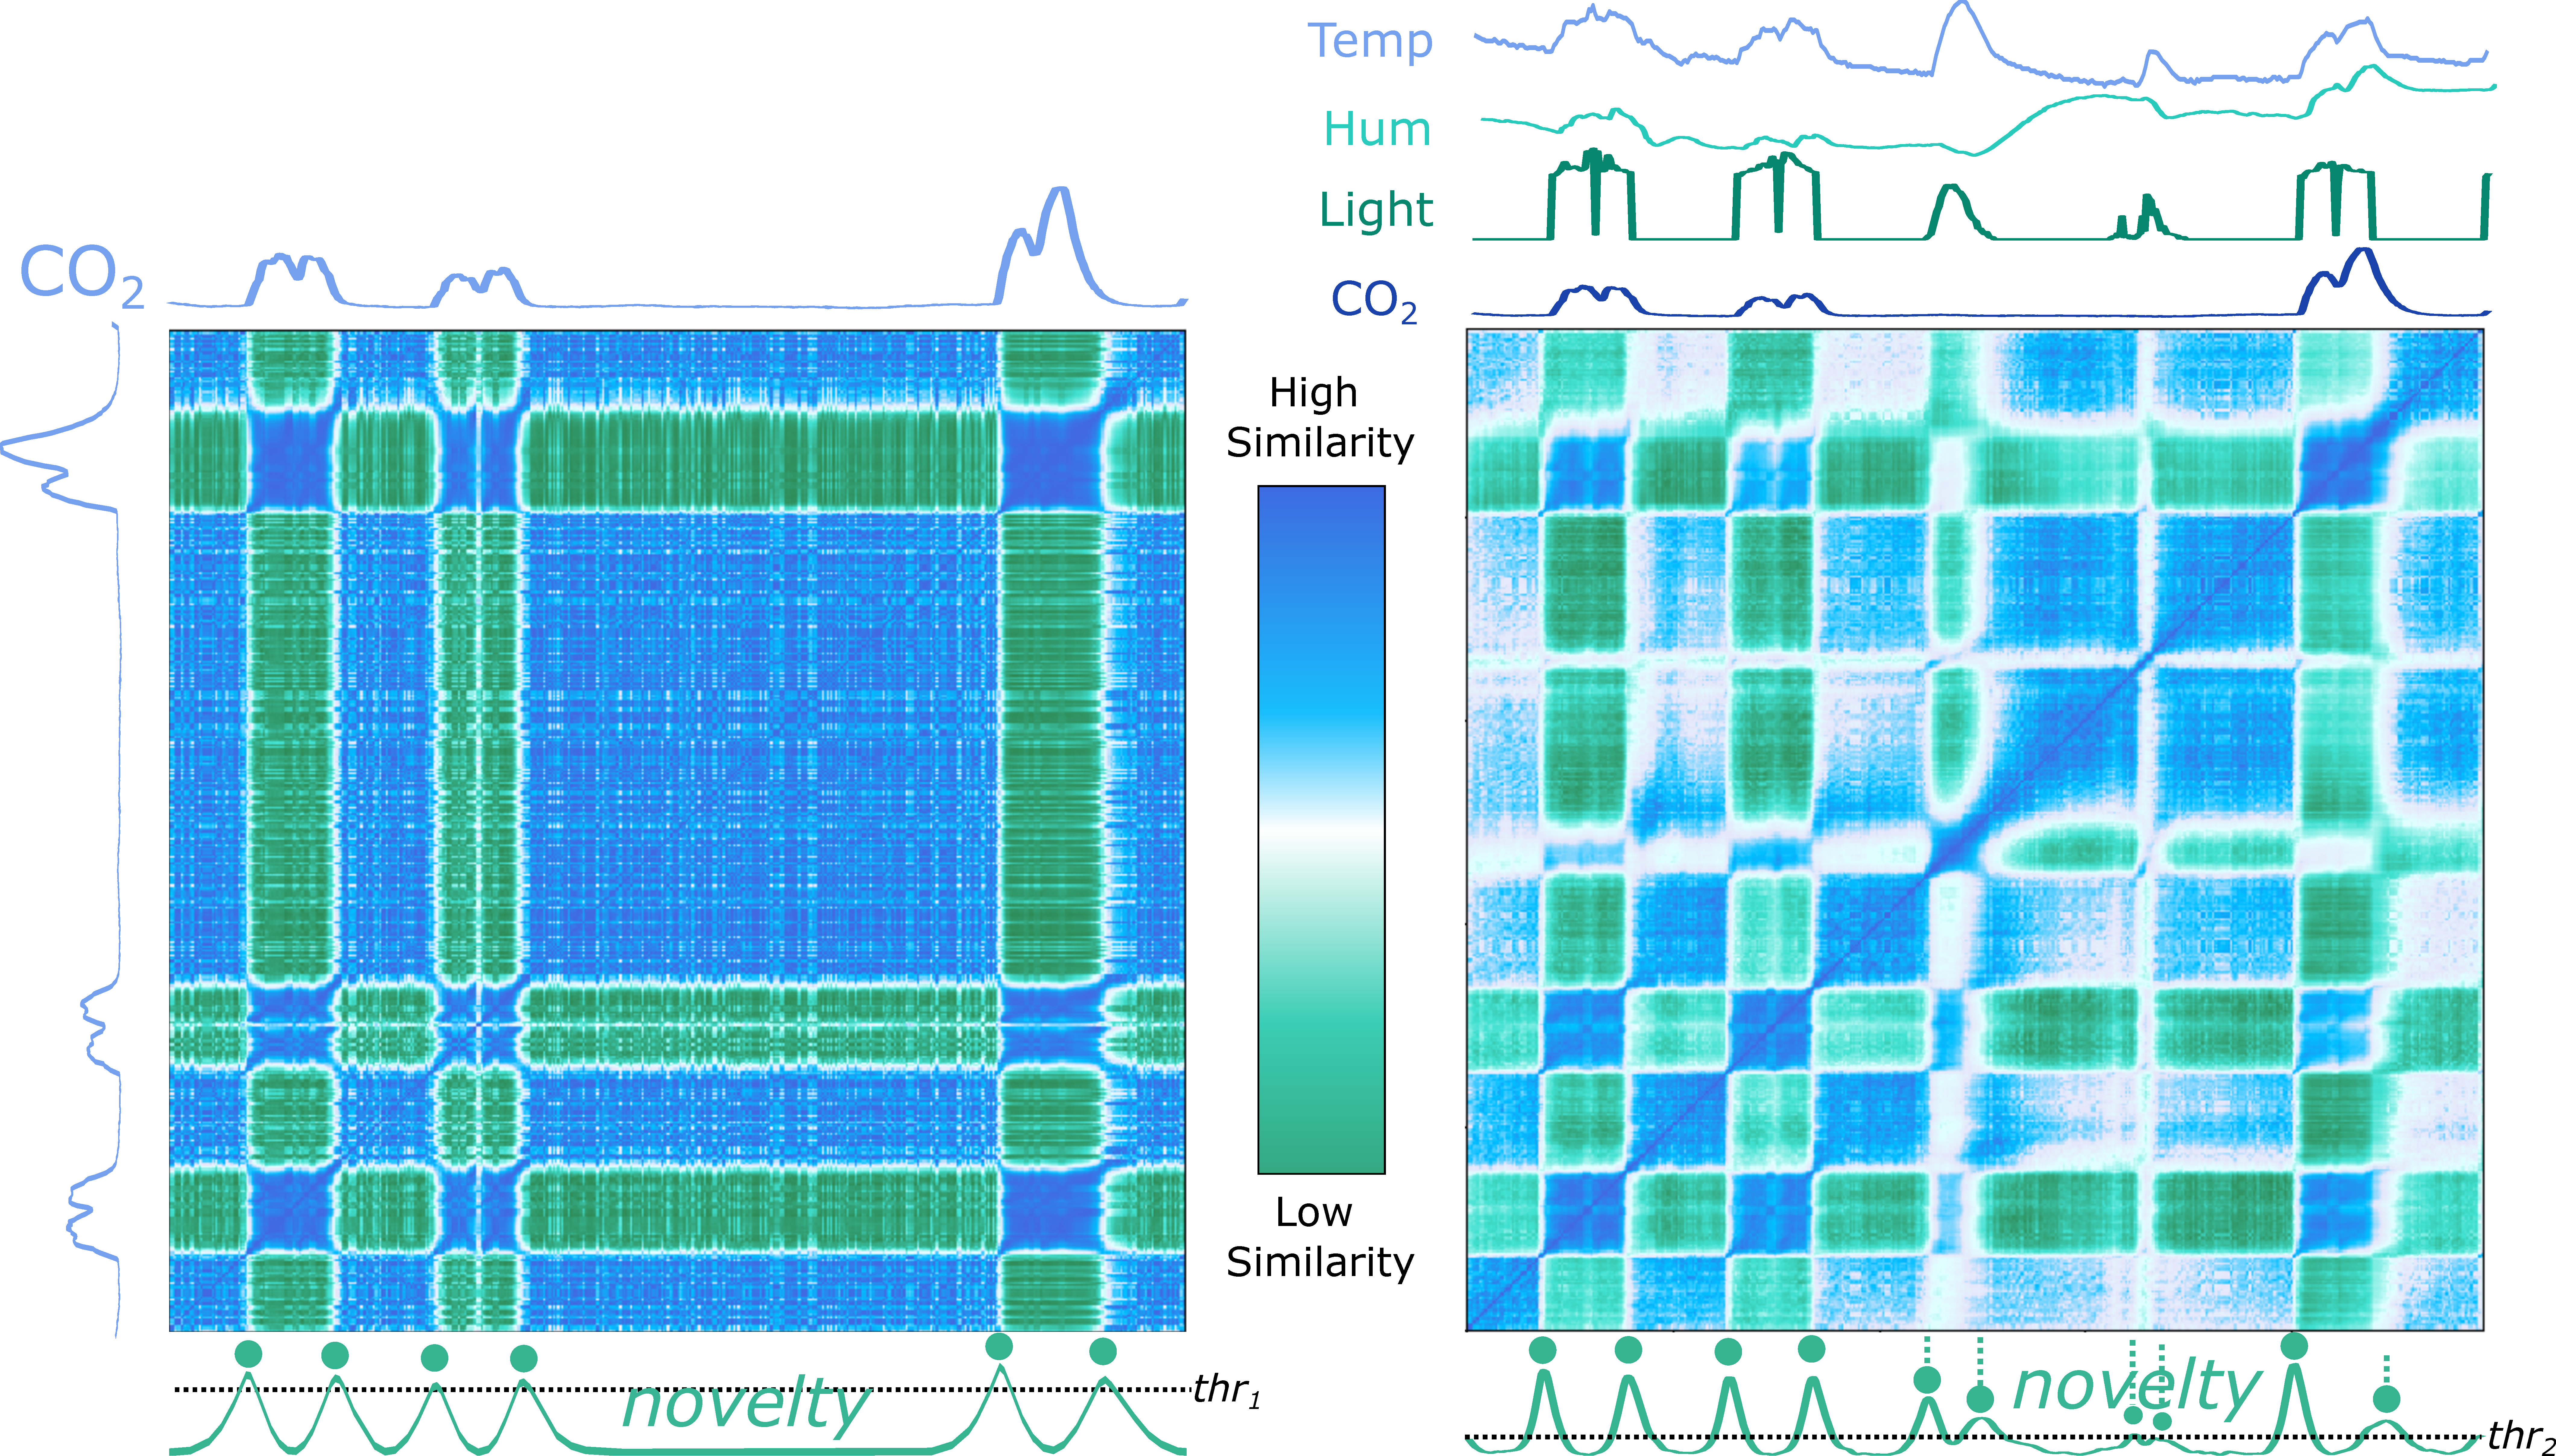
\includegraphics[width=0.9\linewidth]{use_case4_multi.pdf}
    \caption{Proposed method applied on "\textit{Occupancy}" record of Dataset \ref{sec:dataset8}. (a) A single time series of the record is used to extract events; while in (b) the \gls{ssm} is computed with features extracted from the four available time series.}
    \label{fig:example4}
\end{figure}

The proposed method accepts both single and multidimensional records. The difference regards the number of features extracted. As presented in Figure \ref{fig:SSM_scheme}, the same set of features is extracted for each time series of the record and combined in the $F_M$. 
\par
Using a single time series of a multivariate record is optional and depends on the detection's purpose. In some cases, using a single time series from a multidimensional record can lead to missing relevant events undetected. An example of this can be seen on Figure \ref{fig:example4}.a with record \textit{"Occupancy"} from Dataset \ref{sec:dataset8}. 
\par
The record is a multi-dimensional time series that measures room occupancy based on temperature, humidity, light, and $CO_2$. All events can only be detected if using several time series of the record \cite{cpd_alan}. In Figure \ref{fig:example4}.a, a single time series was analyzed by the proposed method to detect relevant events, while Figure \ref{fig:example4}.b is the result of using all the time series of the record.


\section{Time Series Summarization}

The aforementioned examples show how the proposed method can be used as a strong and reliable visual tool. It is possible to see how a time series is structured, how similar are segments, and if these are periodic or not. The information available is quite relevant to support the labeling process of the analyst, but it also can be used to summarize a time series and give a meaningful report about it. 
\par
Following the presented work, we studied how to use it for a meaningful summary of time series. This process is inspired by methodologies that exist in other scenarios for data summarization techniques with statistical analysis, such as the available methods from the \textit{pandas python library}: \textit{pandas.profile()} and \textit{pandas.describe()}. These methods can provide a summarization of a dataset (typically of categorical data) that is given as input. A similar method is not known for time series. In order to develop such a method, we should first understand what is meaningful and relevant to represent as a summary.

\subsection{Elements with Relevance}

In this section, we have been discussing which elements are relevant in time series, mostly associated with \textit{events}. From \textit{events} we can segment homogeneous \textit{subsequences}, recurrent or periodic patterns and anomalies. The relationship between these segments is possible by analyzing their similarity. In addition, a characterization of the segments is possible with statistical analysis. In that sense, the relevant elements to summarize in a time series are (1) \textit{homogeneous segments}, (2) \textit{periodic patterns}, (3) \textit{recurrent patterns}, (4) \textit{anomalies}, (5) association based on similarity and (6) statistical characterization. Several examples from other domains can be used as inspiration on how to join all these elements in a compact, expressive and intuitive way.

\subsection{Compact Design}

Strategies that are typically used to present information compactly are found in several domains. In text analysis, for instance, the relationship between repeating sequences is illustrated with arc diagrams \cite{bitmap, arcplots}. These show where repeating sequences occur in a very concise way. This has a range of applications that include, for example, text and \textit{DNA} sequence analysis.


% One domain that has interesting examples in data visualization is \textit{genomics}. Graphical genome maps are found to concatenate a significant amount of information in a very compact way. Genome features and sequence characteristics are assessed with this visual strategy. An example can be found in Figure \ref{fig:genomic2}. This type of visualization inspired the summarization approach proposed for time series.
\par
This visualization strategy has several elements that can be used to transform the \gls{ssm} into a compact form of filtered information. The elements are (1) multi-layered colored \textit{segments}, (2) \textit{chords} that connect to nearest neighbor \textit{segments} and (3) circular signals on top of segments. The transformation into this compact representation can be performed with the explained analysis methods above.

\subsection{A step by step example}

\begin{figure}
\centering
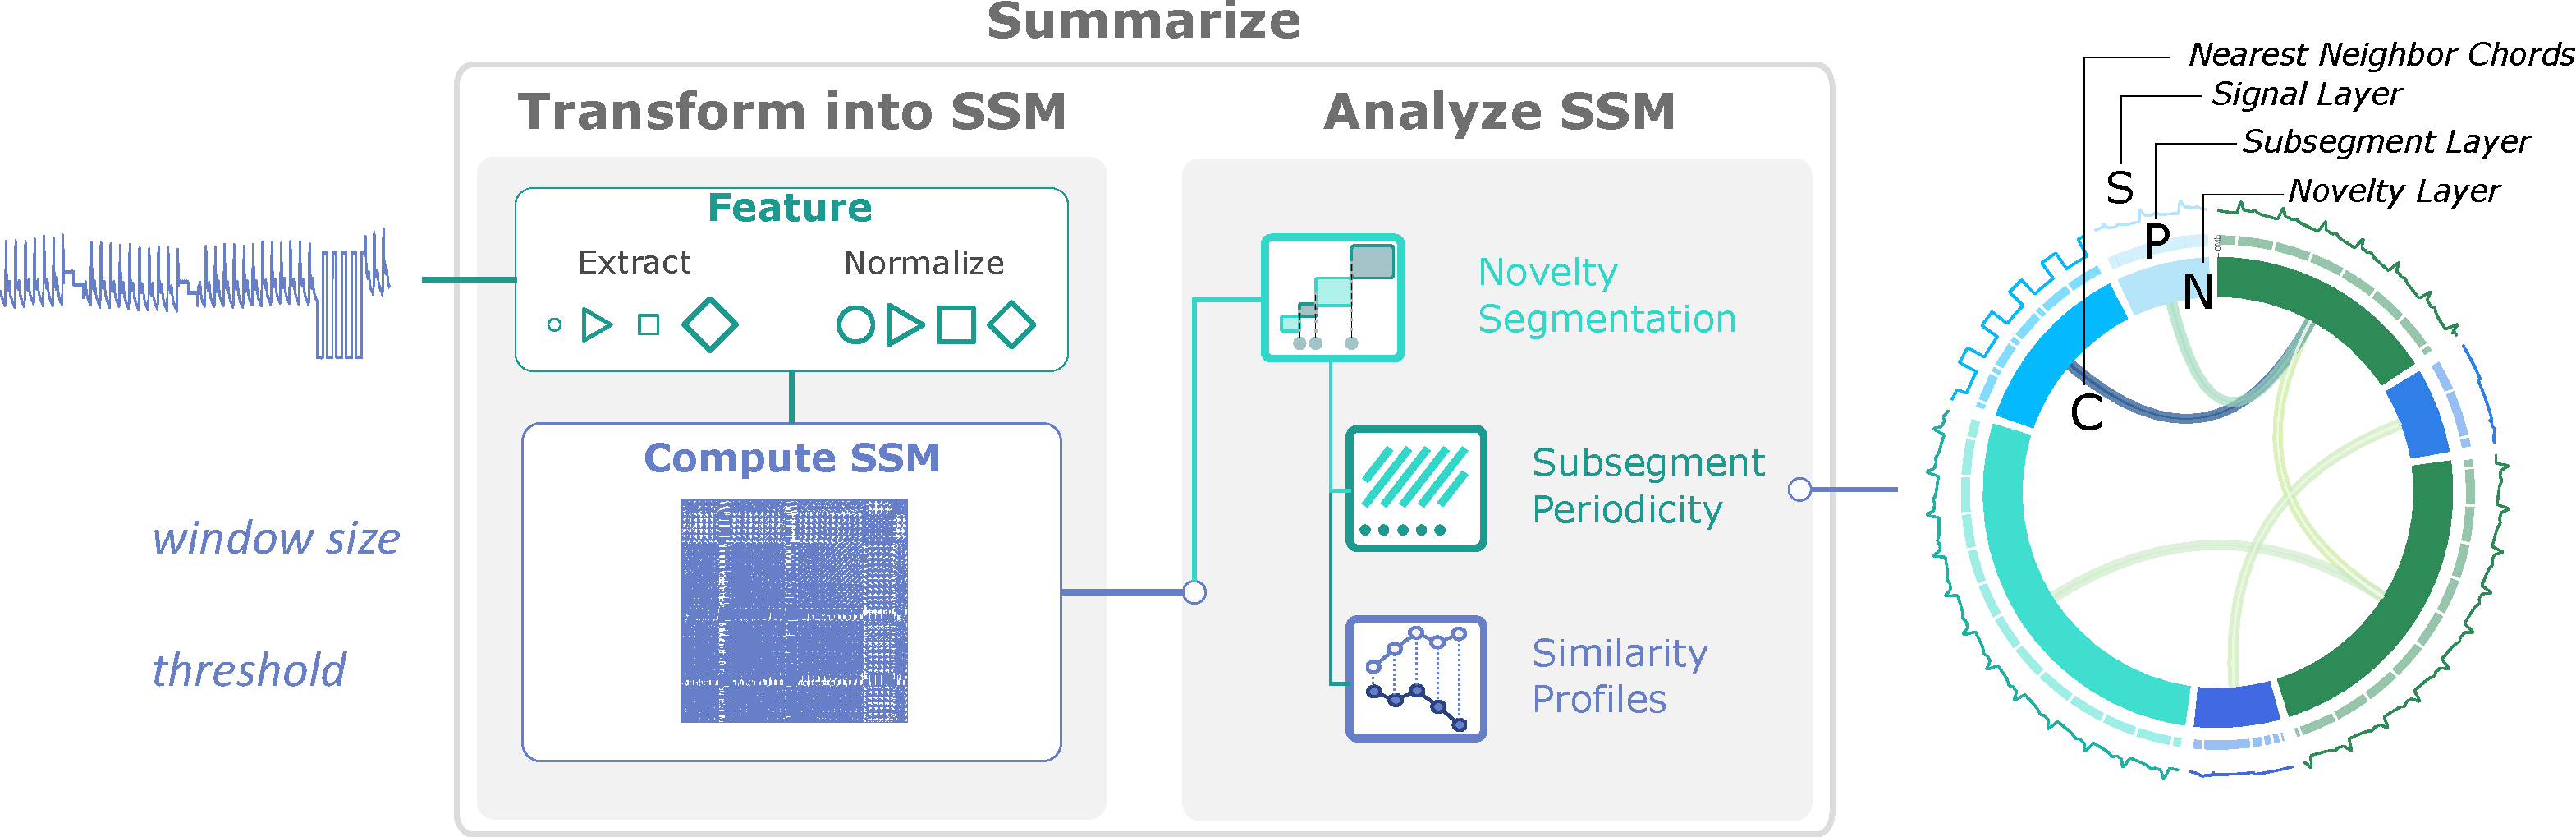
\includegraphics[width=\linewidth]{summarize_steps.pdf}
\caption{Steps to use the aforementioned methods on the \gls{ssm} to summarize the time series into a circular plot with C - chords that connect nearest neighbors, S - the signal layer, P - the subseqment layer and N - the color coded novelty layer. Each of these elements of the summarized plots are built based on novelty segmentation, subsegment periodicity check and similarity profiles.}
\label{fig:summarize_steps}
\end{figure}

The steps are indicated in Figure \ref{fig:summarize_steps} for the \gls{abp} signal example. After computing the \gls{ssm}, it is firstly analyzed to segment the signal based on the \textit{nova} function. These segments are then compared based on the \textit{similarity profiles}. Additional layers can be created by performing an iterative and multi-scale segmentation. With this process, the time series is segmented (\textit{novelty layer}), subsegmented (\textit{subsegment layer}), each segment is connected to the nearest neighbor segment (\textit{nearest neighbor chords}) and the colors for each segment is given based on their similarity to the first segment. Figures \ref{fig:summarize_step1}, \ref{fig:summarize_step2} and \ref{fig:summarize_step3} show the step-by-step process to summarize the time series by analyzing the \gls{ssm}. 

\begin{figure}
\centering
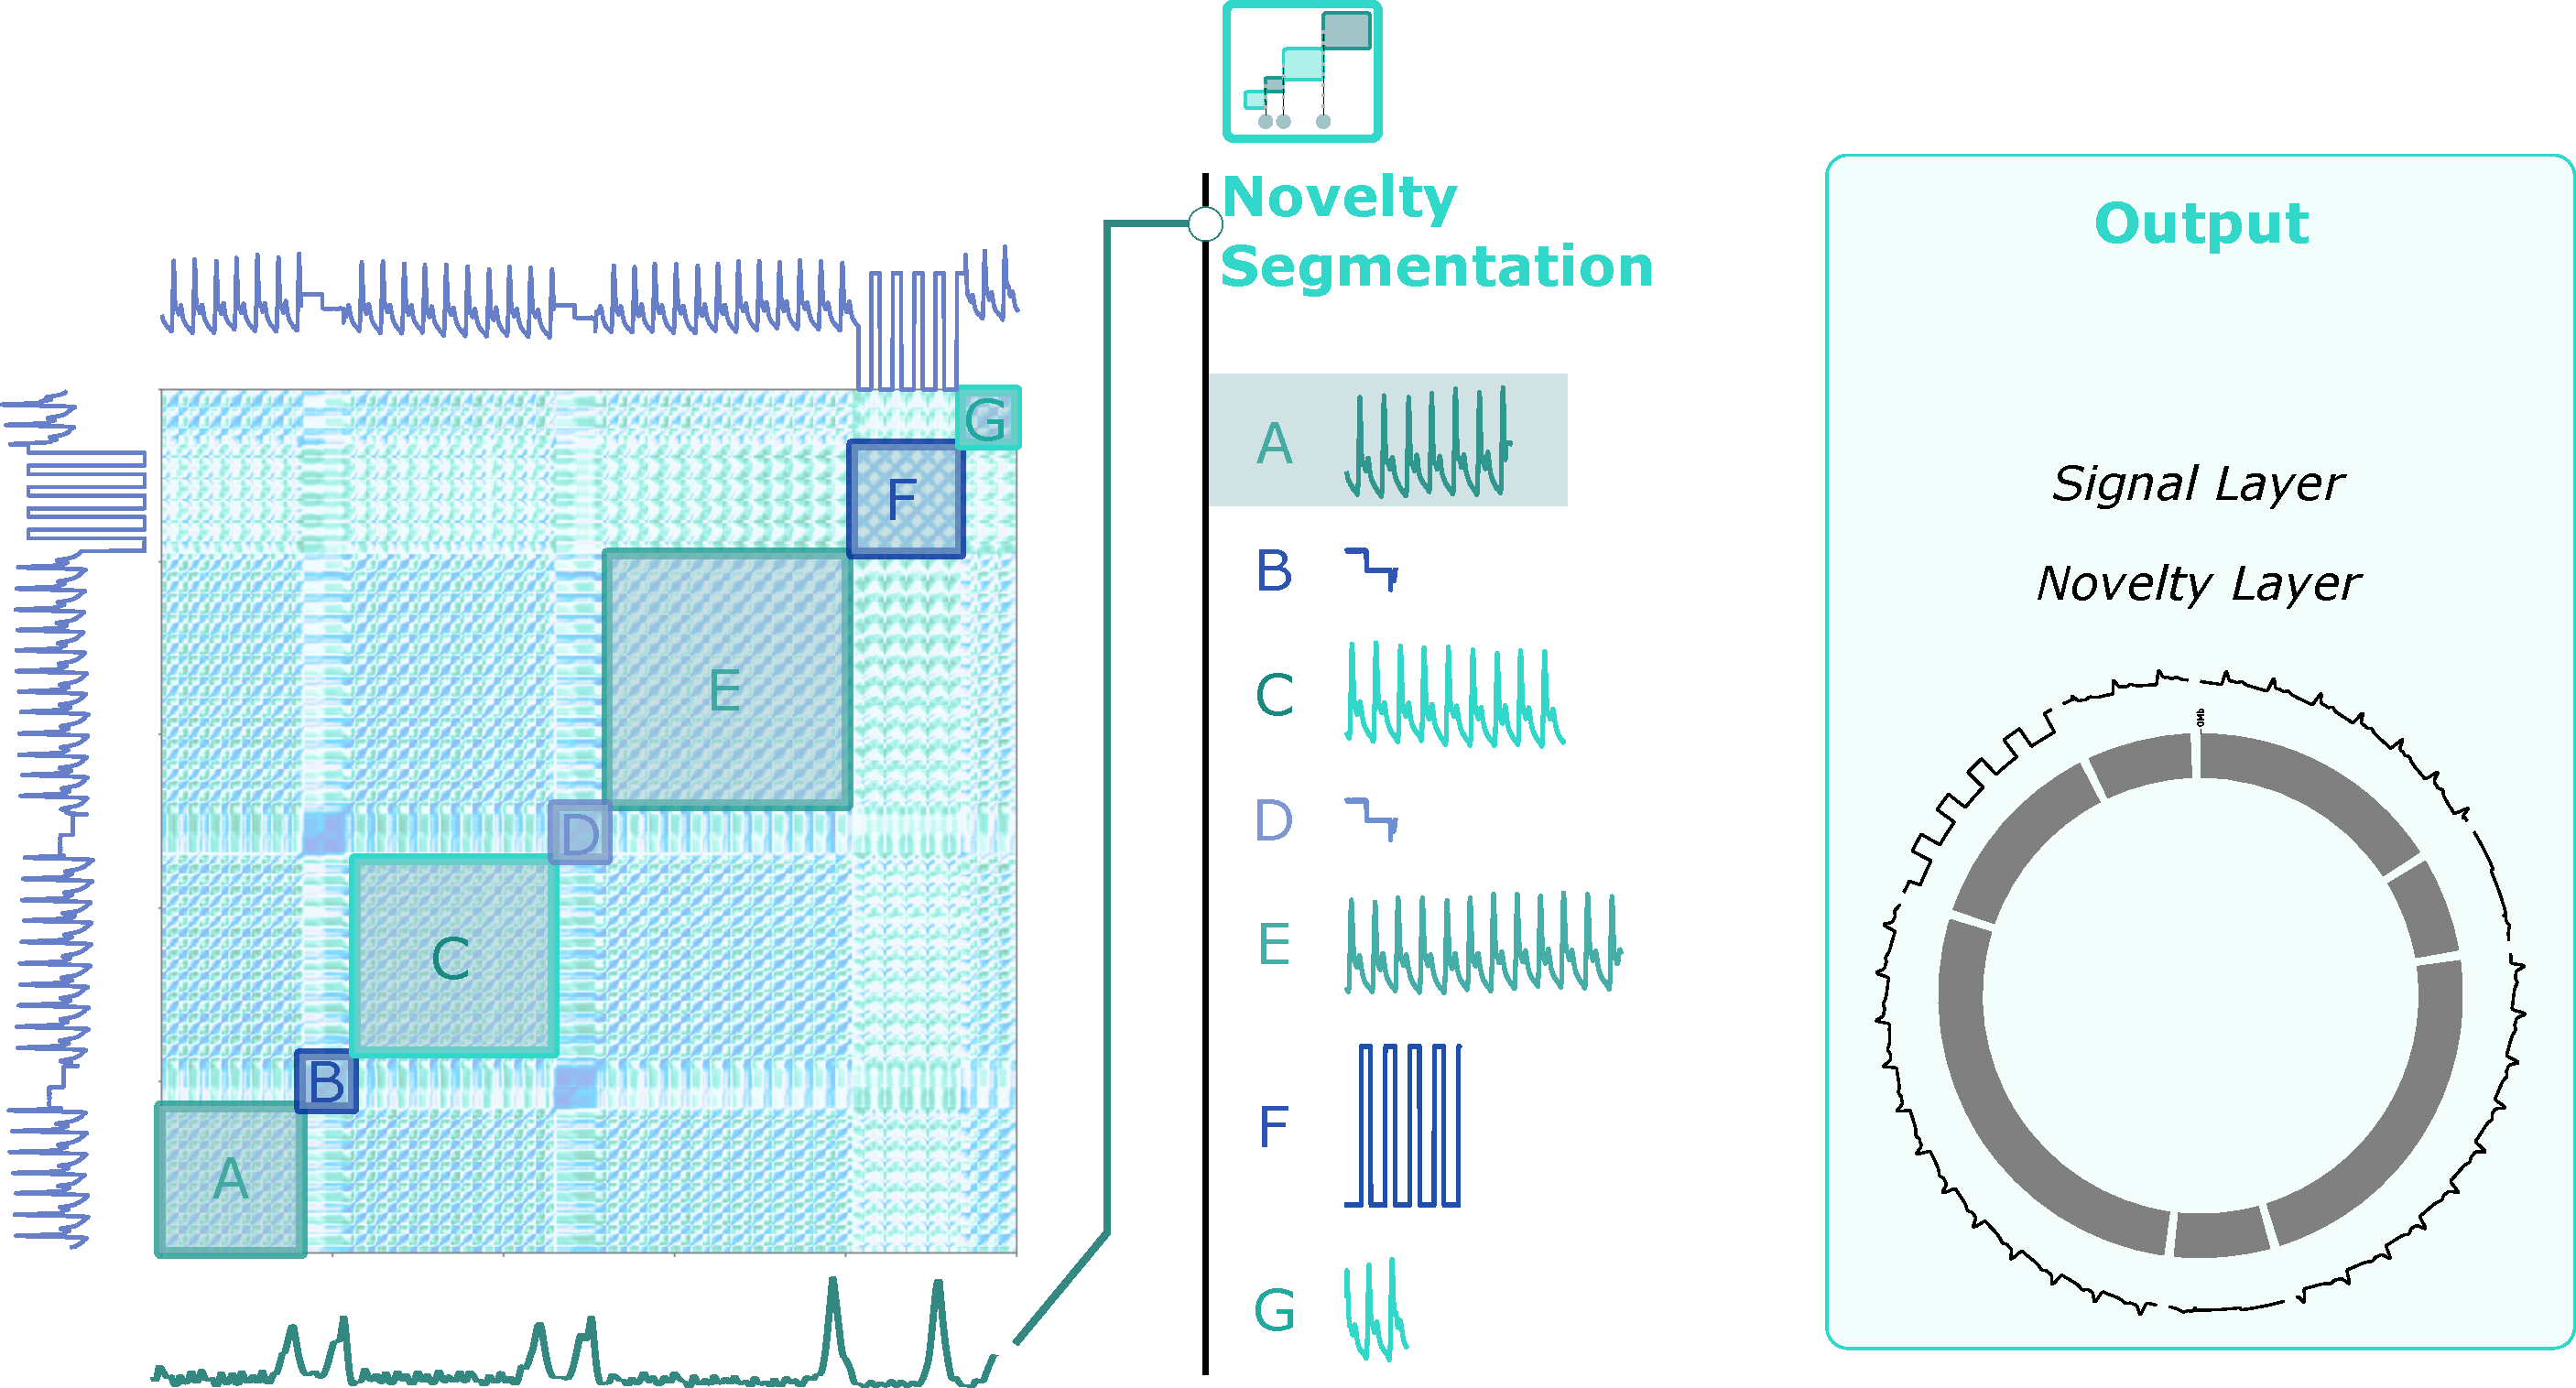
\includegraphics[width=0.85\linewidth]{summarize_step1.pdf}
\caption{How to reach a standard format. This step applies the novelty search method to find the segmentation points. The signal is broken into A to G segments.}
\label{fig:summarize_step1}
\end{figure}

The \textit{nova} function segments the time series into seven segments. The reader can notice that segments A, C, E, and G are similar and separated by segments B, C and F, represented by a failure in the connection of the sensor. From this first segmentation, the \textit{novelty layer} is created, indicating how structured is the signal, as presented in Figure \ref{fig:summarize_step1}.

\begin{figure}[b]
\centering
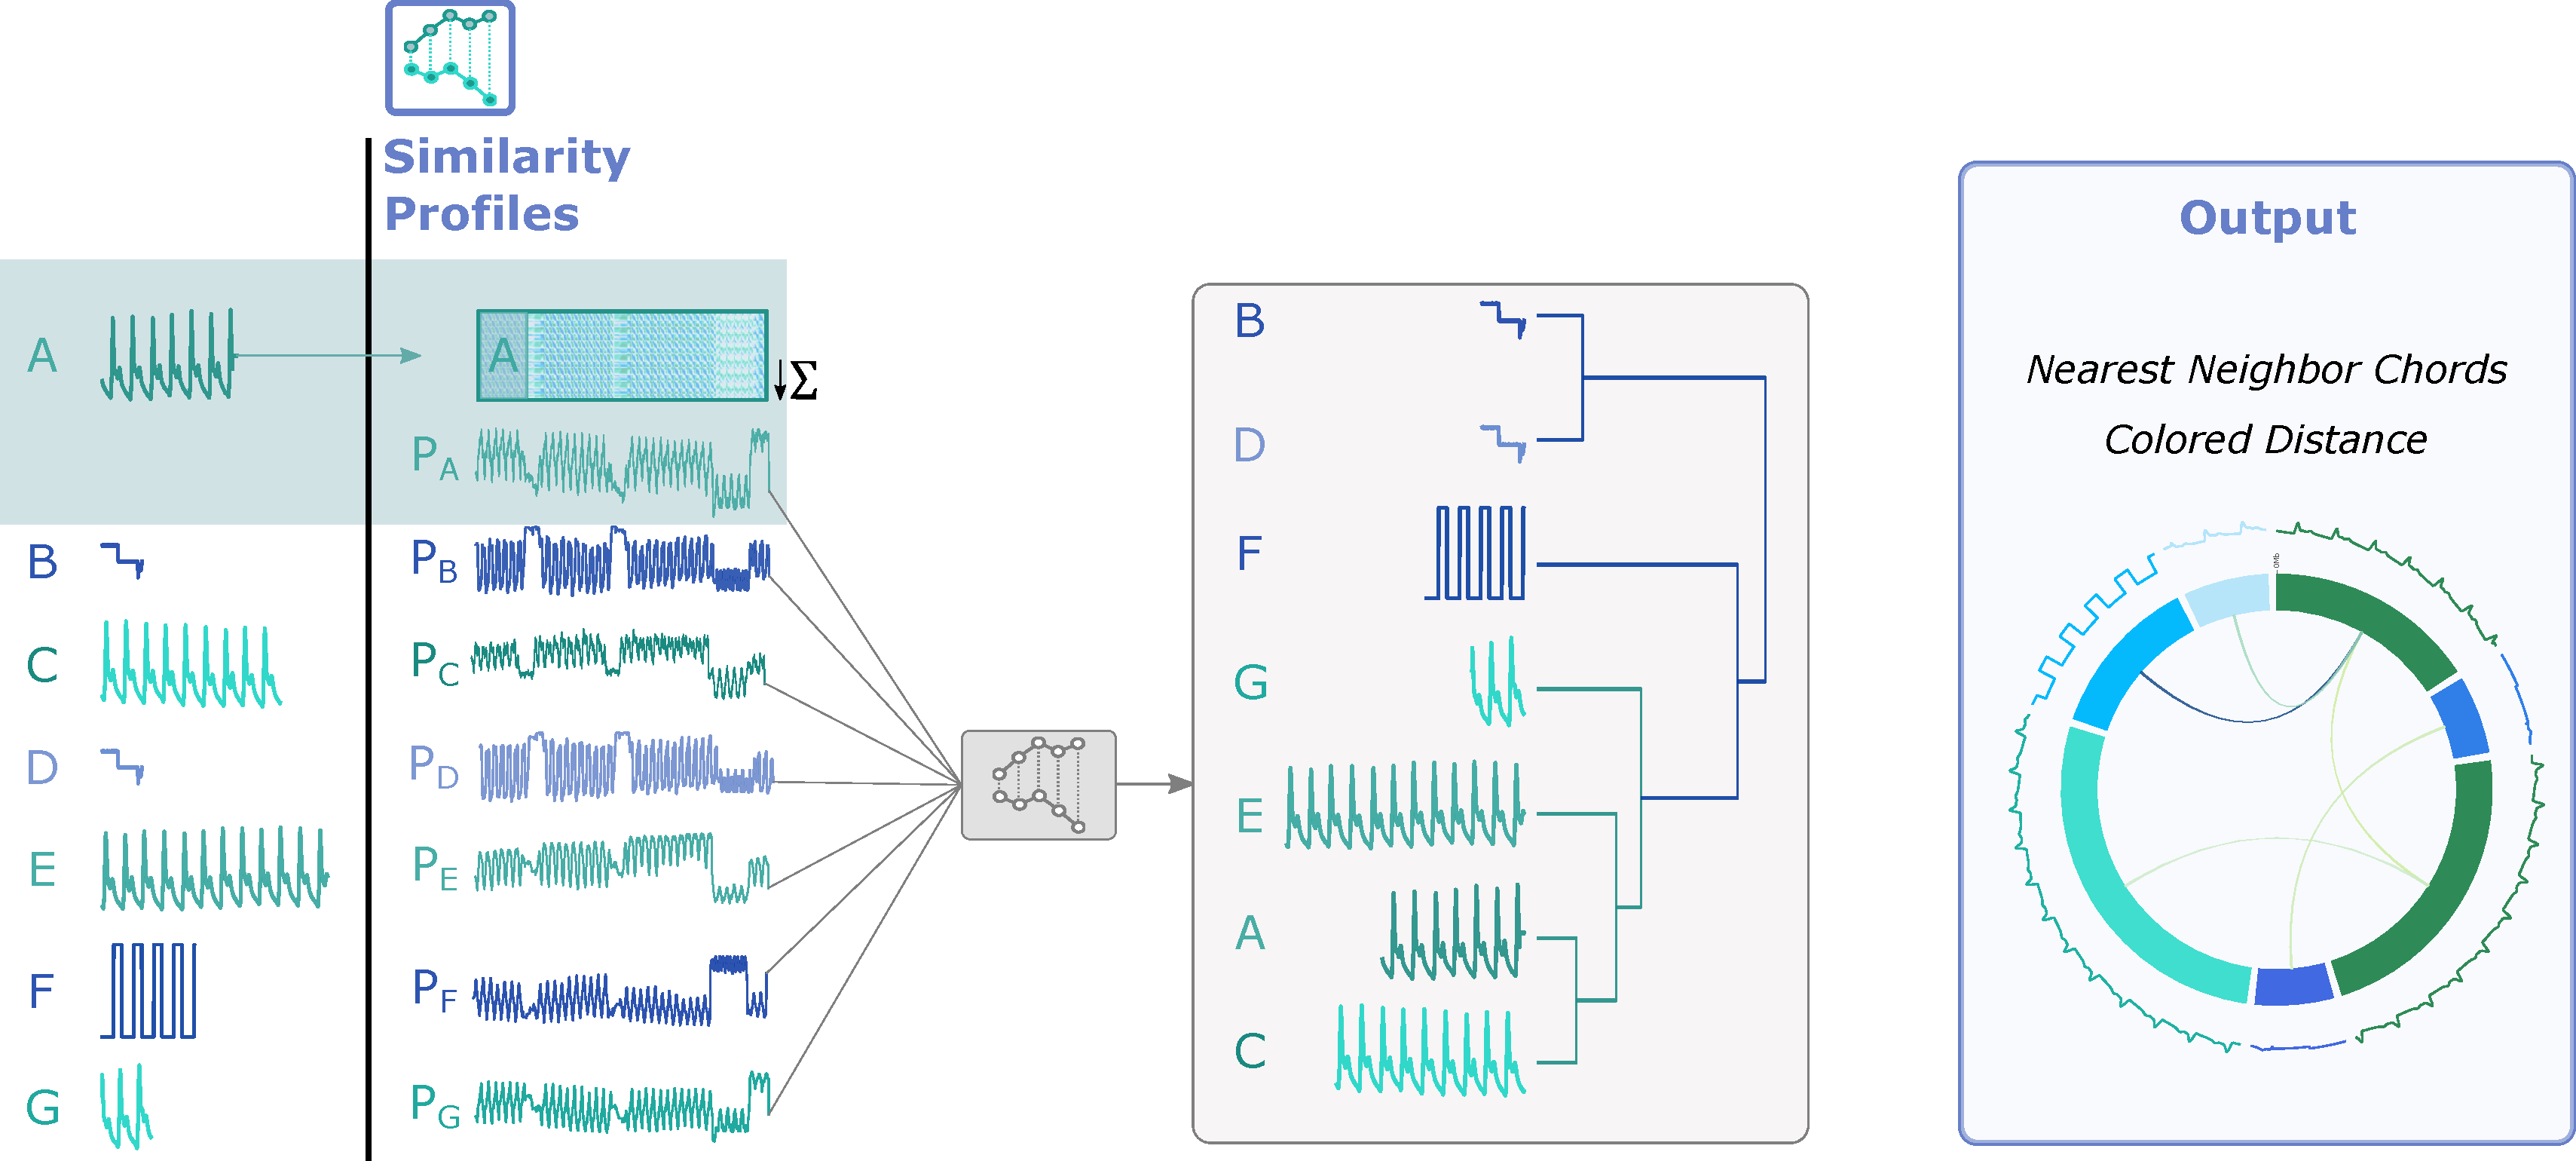
\includegraphics[width=\linewidth]{summarize_step2.pdf}
\caption{From each segment, a similarity profile can be computed. The pairwise euclidean distance is applied to these profiles, from which a dendogram is created. From this association, layer C can be drawn and the colors of the novelty layer can be added. Segment A is highlighted for the next step.}
\label{fig:summarize_step2}
\end{figure}

Further, the segments are compared with the \textit{similarity profiles} of each segment. Figure \ref{fig:summarize_step2} illustrates as example the rows of the \gls{ssm} delimited by segment A and the column-wise average into $P_A$. The same process is applied to each segment. From this Figure, the reader may notice that the profiles $P_A$, $P_C$, $P_E$, and $P_G$ are more similar, while profiles $P_B$ and $P_D$ are more similar as well. The pairwise distance is computed between profiles, which can then be used to extract the nearest neighbor of each segment, as well as transform the distance values between segments into color. 
\par
The pairwise distance between profiles is also used to illustrate how the segments are ordered and clustered by the dendrogram of Figure \ref{fig:summarize_step2}. The dendrogram shows that there are three main clusters, being cluster one represented by segments A, C, E, and G; the second cluster has segment F and the third cluster groups segments B and D. It is important to note that typical distance measures, such as the \gls{ed} or \gls{dtw}, would not be able to directly sort these segments correctly. Using \textit{similarity profiles} is more robust and invariant to the size and time distortions. 

\begin{figure}
\centering
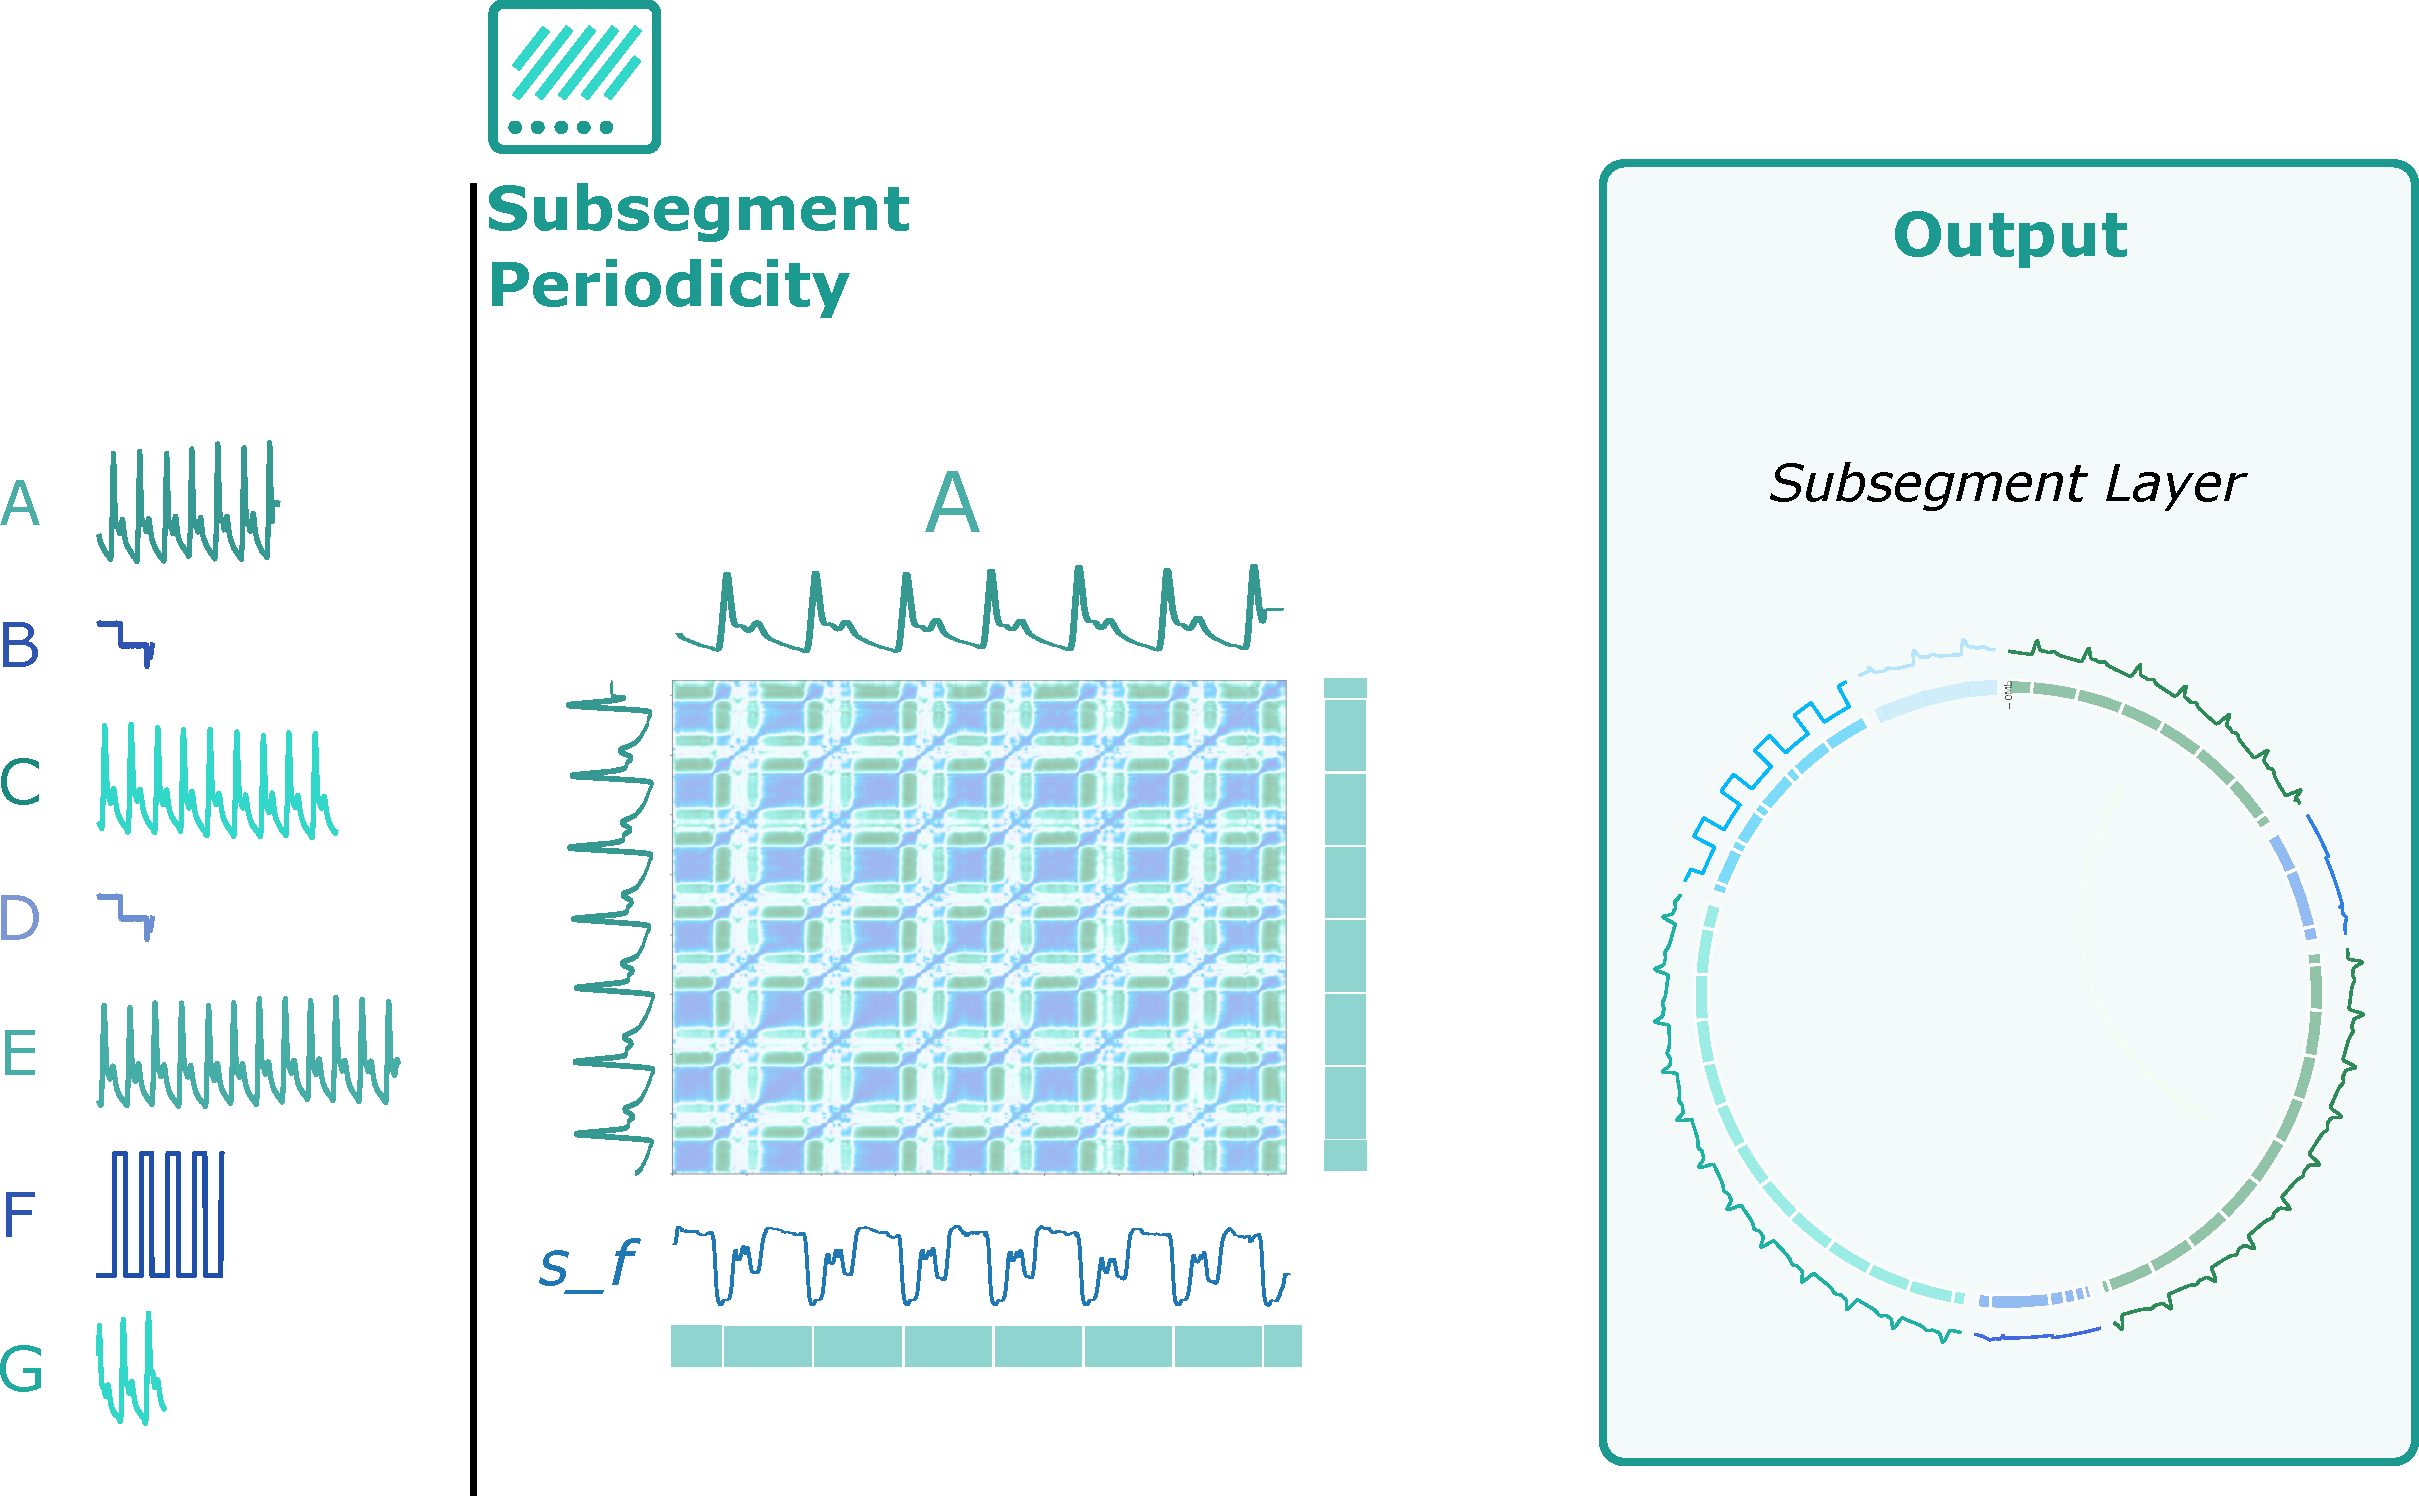
\includegraphics[width=0.75\linewidth]{summarize_step3.pdf}
\caption{After finding the first layer of the segmentation points, the periodicity of each segment can be checked and added as a sublayer of segments, adding layer P. In this case, segment A is the example.}
\label{fig:summarize_step3}
\end{figure}

Finally, the process to summarize the time series can be iterative by adding \textit{subsegment layers}. These layers can be added by performing the \textit{novelty search} on the previously segmented time series with a smaller time scale or segmenting the time series based on periodicity. In this case, the signal is periodic, therefore Figure \ref{fig:summarize_step3} illustrates the \textit{periodic search}, where periods are segmented by the minima of the $s_f$.
\par
This summarization process is mostly graphical and follows the results of each process for information retrieval from the \gls{ssm}. Therefore, this method will not present overall results or be validated in Chapter \ref{cha:results}.
